% =============================================================================
% SEAL-DSA DISSERTATION — Central University of Kashmir
% Department of Information Technology
% =============================================================================
% COMPILER: Use pdfLaTeX (default on Overleaf). 
% If Times New Roman rendering is imperfect, switch compiler to XeLaTeX in 
% Overleaf (Menu → Compiler → XeLaTeX) and uncomment the fontspec lines below.
% =============================================================================
% LOGO: the university logo is included from "image.png", which must be
% uploaded to the Overleaf project root. It appears on the Cover page,
% Title page (width=3cm) and Certificate (width=2.5cm). Adjust the width
% values if the logo renders too large or too small.
% =============================================================================

\documentclass[12pt,a4paper]{report}

% -------------------- Encoding & Fonts --------------------
\usepackage[T1]{fontenc}
\usepackage[utf8]{inputenc}
\usepackage{mathptmx}          % Times New Roman equivalent
\usepackage{setspace}            % Double spacing
\doublespacing

% Uncomment the next 3 lines ONLY if you switch Overleaf compiler to XeLaTeX:
% \usepackage{fontspec}
% \setmainfont{Times New Roman}
% \setmonofont{Courier New}

% -------------------- Page Layout --------------------
\usepackage{geometry}
\geometry{
    left=2.5cm,
    right=2.0cm,
    top=2.0cm,
    bottom=2.0cm,
    headheight=14pt
}

% -------------------- Paragraph Settings --------------------
\usepackage{parskip}
\setlength{\parindent}{0pt}
\setlength{\parskip}{0.5em}

% -------------------- Headings Formatting --------------------
\usepackage[explicit]{titlesec}
\usepackage{ulem}

% Chapter: 20pt, Centered, Bold, 30pt above and below
\titleformat{\chapter}[display]
    {\normalfont\fontsize{20}{24}\selectfont\bfseries\centering}
    {\chaptertitlename\ \thechapter}{20pt}
    {\fontsize{20}{24}\selectfont #1}
\titlespacing*{\chapter}{0pt}{30pt}{30pt}

% Section (Paragraph Heading): 14pt, Underlined, Left Aligned, Bold
\titleformat{\section}
    {\normalfont\fontsize{14}{16}\selectfont\bfseries}
    {\thesection}{1em}{\uline{#1}}

% Subsection: 12pt, Bold
\titleformat{\subsection}
    {\normalfont\fontsize{12}{14}\selectfont\bfseries}
    {\thesubsection}{1em}{#1}

% -------------------- Page Numbers --------------------
\usepackage{fancyhdr}
\pagestyle{fancy}
\fancyhf{}
\fancyfoot[R]{\thepage}
\renewcommand{\headrulewidth}{0pt}
\renewcommand{\footrulewidth}{0pt}

% -------------------- Floats & Captions --------------------
\usepackage{graphicx}
\usepackage{caption}
\captionsetup[table]{
    position=above,
    font=small,
    justification=raggedright,
    singlelinecheck=false,
    labelsep=colon
}
\captionsetup[figure]{
    position=below,
    font=small,
    justification=centering,
    labelsep=colon
}

% -------------------- Code Listings --------------------
\usepackage{listings}
\usepackage{xcolor}
\lstset{
    basicstyle=\fontfamily{pcr}\selectfont\fontsize{10}{12}\selectfont,
    breaklines=true,
    frame=single,
    numbers=left,
    numberstyle=\tiny\color{gray},
    keywordstyle=\bfseries,
    commentstyle=\itshape,
    showstringspaces=false,
    tabsize=4
}

% -------------------- Algorithms --------------------
\usepackage{algorithm}
\usepackage{algpseudocode}

% algpseudocode has no try/end-try block; define one.
\algblockdefx[TRY]{Try}{EndTry}{\textbf{try}}{\textbf{end try}}

% listings has no built-in JSON language; define a minimal one.
\lstdefinelanguage{json}{
    morestring=[b]",
    morecomment=[l]{//},
    morecomment=[s]{/*}{*/},
    sensitive=false,
}

% -------------------- Tables --------------------
\usepackage{booktabs}
\usepackage{array}
\usepackage{longtable}
\usepackage{adjustbox}
\usepackage[section]{placeins}  % floats stay within their own section
\usepackage{pgfplots}          % result charts drawn natively from the run data
\pgfplotsset{compat=1.18}
\setlength{\tabcolsep}{4pt}     % tighter columns so wide tables fit the text block

% Verbatim (ASCII diagrams) at 10pt Courier, per the code-snippet guideline.
% At 12pt the wider diagrams overrun the right margin.
\makeatletter
\renewcommand{\verbatim@font}{\normalfont\ttfamily\fontsize{10}{12}\selectfont}
\makeatother

% -------------------- Float placement & widow control --------------------
% Prevents near-empty pages caused by floats pushing text, and single stranded
% lines at the top or bottom of a page.
\widowpenalty=10000
\clubpenalty=10000
\renewcommand{\topfraction}{0.85}
\renewcommand{\bottomfraction}{0.70}
\renewcommand{\textfraction}{0.10}
\renewcommand{\floatpagefraction}{0.75}
\setcounter{topnumber}{3}
\setcounter{bottomnumber}{2}
\setcounter{totalnumber}{4}

% -------------------- Math --------------------
\usepackage{amsmath}
\usepackage{amssymb}
\usepackage{amsfonts}

% -------------------- Misc --------------------
\usepackage{enumitem}
\usepackage{verbatim}
\usepackage{alltt}
\usepackage{hyperref}
\hypersetup{colorlinks=true,linkcolor=black,citecolor=black,urlcolor=blue}

% -------------------- Custom Commands --------------------
\newcommand{\code}[1]{\texttt{#1}}

% =============================================================================
% BEGIN DOCUMENT
% =============================================================================
\begin{document}

% Front matter carries no page numbers; numbering begins at the Main Report.
\pagestyle{empty}

% -------------------- COVER PAGE (no page number) --------------------
\thispagestyle{empty}
\begingroup
\singlespacing
\begin{center}

\vspace*{0.5cm}

\includegraphics[width=3.2cm]{image.png}\\[0.9cm]

{\fontsize{19}{24}\selectfont\bfseries SEAL-DSA: A Self-Adapting Language Model for Autonomous Improvement in Data Structures and Algorithms Education\par}

\vfill

Submitted by\\[0.6cm]
{\large\bfseries Taqaddus Shafi\par}
\vspace{0.2cm}
{\normalsize Registration No.~2402cukrm04\par}

\vfill

In the partial fulfillment of the requirement for the award of degree of\\[0.15cm]
Master of Technology in Computer Science \& Engineering\\[0.15cm]
(M.~Tech.~CSE)

\vfill

Submitted To\\[0.6cm]
Department of Information Technology\\[0.15cm]
School of Engineering \& Technology\\[0.15cm]
Central University of Kashmir\\[0.15cm]
Ganderbal, J\&K.

\vfill

{\large\bfseries 2026\par}

\vspace*{0.5cm}

\end{center}
\endgroup
\clearpage

% -------------------- TITLE PAGE (no page number) --------------------
\thispagestyle{empty}
\begingroup
\singlespacing
\begin{center}

\vspace*{0.5cm}

\includegraphics[width=3.2cm]{image.png}\\[0.9cm]

{\fontsize{19}{24}\selectfont\bfseries SEAL-DSA: A Self-Adapting Language Model for Autonomous Improvement in Data Structures and Algorithms Education\par}

\vfill

Submitted By\\[0.6cm]
{\large\bfseries Taqaddus Shafi\par}
\vspace{0.2cm}
{\normalsize Registration No.~2402cukrm04\par}

\vfill

In partial fulfillment of the requirement for the award of degree of\\[0.15cm]
MASTER OF TECHNOLOGY IN\\[0.15cm]
COMPUTER SCIENCE \& ENGINEERING\\[0.15cm]
(M.~Tech.~CSE)

\vfill

Submitted To\\[0.6cm]
Department of Information Technology\\[0.15cm]
School of Engineering \& Technology\\[0.15cm]
Central University of Kashmir\\[0.15cm]
Ganderbal, J\&K.

\vfill

{\large\bfseries 2026\par}

\vspace*{0.5cm}

\end{center}
\endgroup
\clearpage

% -------------------- CERTIFICATE --------------------
\thispagestyle{empty}
\begingroup
\singlespacing
\begin{center}
\includegraphics[width=2.5cm]{image.png}\\[0.6cm]
\end{center}

\begin{center}
Ref No. : \dotfill\\
Date: \dotfill
\end{center}

\vspace{0.3cm}

\noindent Department of Information Technology\\
School of Engineering \& Technology\\
Central University of Kashmir\\
Ganderbal, J\&K.

\vspace{0.6cm}

\begin{center}
{\large\bfseries CERTIFICATE}
\end{center}

\vspace{0.4cm}

This is to certify that the project titled ``SEAL-DSA: A Self-Adapting Language Model for Autonomous Improvement in Data Structures and Algorithms Education'' has been carried by:

\begin{center}
\textbf{Mr.~Taqaddus Shafi}\\[0.2cm]
Registration No.~2402cukrm04
\end{center}

under my supervision, in the partial fulfillment of the requirement for the award of degree of Master of Technology in Computer Science \& Engineering (M.~Tech.~CSE) during the academic year 2026.

\vspace{1cm}

\noindent Supervisor:\\[0.4cm]
\textbf{Zahoor Ahmad Najar}\hfill\textbf{Head}\\
Assistant Professor,\\
Department of Information Technology

\vspace{1cm}

Certified that I have examined the project titled ``SEAL-DSA: A Self-Adapting Language Model for Autonomous Improvement in Data Structures and Algorithms Education'' on \underline{\hspace{3cm}} \underline{\hspace{3cm}}.

\vspace{1cm}

\hfill\textbf{External Examiner}
\endgroup

\clearpage

% -------------------- ACKNOWLEDGEMENT --------------------
\chapter*{Acknowledgement}
\addcontentsline{toc}{chapter}{Acknowledgement}
\begingroup
\singlespacing

The completion of this dissertation would not have been possible without the support and guidance of a number of people, and it is a pleasure to record my gratitude to them here.

I am deeply indebted to my supervisor, Zahoor Ahmad Najar, Assistant Professor, Department of Information Technology, for accepting me as a student and for the guidance provided throughout the course of this work.

I express my sincere thanks to the Head, Department of Information Technology, and to the entire faculty of the School of Engineering \& Technology, Central University of Kashmir, for providing the academic environment and the infrastructure that made this work possible.

I gratefully acknowledge the open-source community whose work this project is built upon. In particular, the Qwen team at Alibaba Cloud for releasing the Qwen2.5 model family under a permissive licence, and the maintainers of the HuggingFace Transformers, PEFT, and bitsandbytes libraries, without which parameter-efficient training on freely available hardware would not be feasible for a student project. I also acknowledge Google Colaboratory, whose free tier provided the entire computational budget for this work.

I thank my classmates in the M.~Tech. programme for the many discussions that clarified my thinking over the course of this work.

Finally, I thank my family for their patience and support over the duration of this work.

\vspace{1cm}

\noindent\textbf{Taqaddus Shafi}\\
\textbf{Reg.~No.~2402cukrm04}
\endgroup

\clearpage

% -------------------- PLAGIARISM UNDERTAKING --------------------
\chapter*{Plagiarism Undertaking}
\addcontentsline{toc}{chapter}{Plagiarism Undertaking}
\begingroup
\singlespacing

I solemnly declare that research/Project work presented in the dissertation titled ``SEAL-DSA: A Self-Adapting Language Model for Autonomous Improvement in Data Structures and Algorithms Education'' is solely my research/Project work. Small contribution/help wherever taken has been duly acknowledged and that complete dissertation has been written by me.

I understand the zero tolerance policy of the Central University of Kashmir towards plagiarism. Therefore I as an Author of the above titled dissertation declare that no portion of my dissertation has been plagiarized and any material used as reference is properly referred/cited.

I undertake that if I am found guilty of any formal plagiarism in the above titled dissertation even after award of degree, the University reserves the right to take action against me as per University norms.

\vspace{2cm}

\noindent Student/Author Signature:\underline{\hspace{5cm}}\\[0.5cm]
Name:\underline{\hspace{6cm}}
\endgroup

\clearpage

% -------------------- LIST OF ABBREVIATIONS --------------------
\chapter*{List of Abbreviations}
\addcontentsline{toc}{chapter}{List of Abbreviations}
\begingroup
\singlespacing

\begin{longtable}{>{\raggedright\arraybackslash}p{3cm} p{10cm}}
\toprule
\textbf{Abbreviation} & \textbf{Expansion} \\
\midrule
\endhead
AI & Artificial Intelligence \\
API & Application Programming Interface \\
AdamW & Adam optimizer with decoupled Weight decay \\
BFS & Breadth First Search \\
BST & Binary Search Tree \\
CPU & Central Processing Unit \\
CSAIL & Computer Science and Artificial Intelligence Laboratory \\
CUDA & Compute Unified Device Architecture \\
DFD & Data Flow Diagram \\
DFS & Depth First Search \\
DP & Dynamic Programming \\
DPO & Direct Preference Optimization \\
DSA & Data Structures and Algorithms \\
EWC & Elastic Weight Consolidation \\
FIM & Fisher Information Matrix \\
FP16 & 16-bit Floating Point \\
GPU & Graphics Processing Unit \\
JSON & JavaScript Object Notation \\
KV & Key--Value (attention cache) \\
LLM & Large Language Model \\
LoRA & Low-Rank Adaptation \\
NF4 & 4-bit NormalFloat \\
NLP & Natural Language Processing \\
PEFT & Parameter-Efficient Fine-Tuning \\
QLoRA & Quantized Low-Rank Adaptation \\
RAG & Retrieval Augmented Generation \\
RAM & Random Access Memory \\
RLHF & Reinforcement Learning from Human Feedback \\
SEAL & Self-Adapting Language model \\
UML & Unified Modeling Language \\
VRAM & Video Random Access Memory \\
YAML & YAML Ain't Markup Language \\
\bottomrule
\end{longtable}
\endgroup

\clearpage

% -------------------- ABSTRACT --------------------
\chapter*{Abstract}
\addcontentsline{toc}{chapter}{Abstract}

Large language models are frozen at the point of deployment. Once training concludes, a model cannot learn from its own mistakes, cannot incorporate knowledge that emerged after its data cutoff, and cannot specialise toward the needs of the users it actually serves, unless it is retrained at a cost that places the procedure beyond the reach of most educational institutions. This dissertation investigates whether that limitation can be relaxed for a narrow domain, using hardware that costs nothing.

This work presents SEAL-DSA, a self-adapting language model for Data Structures and Algorithms education. The system implements a closed autonomous learning loop in which a single model generates its own practice questions for a selected topic, attempts to answer them, evaluates the quality of its own answers using a combination of a rule-based rubric and sandboxed execution of the generated code against test cases, and updates its own parameters from the resulting signal. Adaptation is confined to a low-rank adapter comprising approximately 0.09\% of the model's parameters, and an Elastic Weight Consolidation penalty derived from a diagonal Fisher Information approximation restrains movement in parameters identified as important to previously acquired capability. A curriculum scheduler directs training effort toward topics on which the model has demonstrated weakness. The complete system operates on the free tier of Google Colaboratory using a single NVIDIA T4 GPU, with the base model held in 4-bit NF4 quantization.

The system was evaluated on a held-out set of seventy questions spanning seven DSA topics, comparing the frozen base model against the self-adapted model within a single session so that a paired question-level comparison is valid. Functional correctness, measured as the fraction of held-out test cases passed by generated code, was 0.1111 both before and after the complete five-epoch training run, and no topic recorded a higher pass rate after adaptation. The aggregate composite score rose by 0.32\%, a movement attributable to keyword coverage rather than to correctness, and one that this evaluation set cannot distinguish from sampling variation. The dissertation shows that three of the four scoring components are saturated on the base model before training begins, so the composite could not have registered a substantial gain irrespective of the training outcome. Capability retention, by contrast, was high: 98.6\% of held-out questions scored unchanged or higher after adaptation, a single question regressed, and the largest topic-level decline was 0.0159, indicating that catastrophic forgetting did not occur.

The dissertation reports these findings without inflation. Self-adaptive training at this scale did not improve the functional correctness of generated code, the movement observed in the composite metric is not distinguishable from noise on a set of this size, and the evaluation instrument was saturated in three of four components before training began. The contribution of the work therefore lies in a functioning end-to-end implementation of self-adaptive training under severe resource constraints, in an execution-based evaluation harness for generated algorithmic code, in empirical evidence that low-rank adaptation regularised by EWC preserves prior capability under self-generated training, and in a precise account of why the approach did not deliver more and what would be required to establish whether it can.

\vspace{0.5cm}
\noindent\textbf{Keywords:} Self-adapting language models, continual learning, low-rank adaptation, elastic weight consolidation, catastrophic forgetting, curriculum learning, parameter-efficient fine-tuning, educational artificial intelligence.

\clearpage

% -------------------- TABLE OF CONTENTS --------------------
\tableofcontents
\clearpage

% -------------------- LIST OF TABLES --------------------
\chapter*{List of Tables}
\addcontentsline{toc}{chapter}{List of Tables}
\begingroup
\singlespacing

\begin{longtable}{>{\raggedright\arraybackslash}p{2cm} p{10cm}}
1.1 & Challenges in maintaining deployed language model quality \\
3.1 & Comparison of MIT SEAL and SEAL-DSA \\
3.2 & Full fine-tuning versus low-rank adaptation \\
3.3 & Continual learning methods considered \\
4.1 & Evaluation rubric dimensions and weights \\
4.2 & Curriculum topic ordering \\
5.1 & Memory budget on the T4 GPU \\
5.2 & Colab limitations and adopted mitigations \\
6.1 & Checkpoint directory contents \\
7.1 & Technology stack \\
7.2 & Candidate base models considered \\
7.3 & Training hyperparameters \\
8.1 & Aggregate performance before and after self-adaptive training \\
8.2 & Topic-wise scores before and after self-adaptation \\
8.3 & Paired question-level outcomes \\
8.4 & Efficiency observations \\
10.1 & Software components and versions \\
\end{longtable}
\endgroup

\clearpage

% -------------------- LIST OF FIGURES --------------------
\chapter*{List of Figures}
\addcontentsline{toc}{chapter}{List of Figures}
\begingroup
\singlespacing

\begin{longtable}{>{\raggedright\arraybackslash}p{2cm} p{10cm}}
1.1 & The SEAL four-stage learning loop \\
4.1 & SEAL-DSA system architecture \\
4.2 & Data flow through one SEAL iteration \\
6.1 & Level 0 data flow diagram \\
6.2 & Level 1 data flow diagram \\
6.3 & Use case diagram \\
6.4 & Sequence diagram of one training iteration \\
6.5 & Class diagram of core modules \\
8.1 & Topic-wise performance before and after self-adaptation \\
8.2 & Evaluation metric breakdown \\
8.3 & Paired question-level outcomes \\
9.1 & Training loop console output \\
9.2 & Checkpoint directory on Google Drive \\
9.3 & Evaluation run console output \\
\end{longtable}
\endgroup

\clearpage

% =============================================================================
% MAIN REPORT — Page numbering starts here
% =============================================================================
\pagestyle{fancy}
\pagenumbering{arabic}
\setcounter{page}{1}

\chapter{Introduction}

\section{Background and Motivation}

The last five years have produced a class of language models whose fluency in technical domains would have been difficult to credit a decade ago. Models in the GPT, Gemini, and LLaMA families answer questions about algorithms, write working code, and explain their reasoning at a standard that is often adequate for an undergraduate audience. Yet all of them share a structural limitation that is rarely stated as prominently as their capabilities: they are frozen at the moment of deployment. The weights that ship are the weights that remain. A deployed model cannot learn from an interaction, cannot repair an error it has been shown to make repeatedly, and cannot acquire knowledge that did not exist when its training data was assembled.

In general-purpose applications this limitation is tolerable, because the vendor periodically retrains and releases a successor. In educational applications it is considerably more damaging, for four reasons.

First, knowledge in a technical discipline evolves. New algorithms are published, complexity bounds are improved, and the practices that are considered idiomatic in a programming language shift over time. A frozen model teaches what was current at its cutoff.

Second, learners differ. The explanation that unlocks a concept for one student is the explanation that confuses another, and a model that cannot adapt cannot discover which explanations work.

Third, errors persist and compound. A model that consistently mis-states the space complexity of an algorithm will mis-state it in every session, to every student, indefinitely. There is no mechanism by which the error self-corrects.

Fourth, and most consequentially for an institution rather than a vendor, the cost of the remedy is prohibitive. Full fine-tuning of even a moderately sized model demands multi-GPU infrastructure, and the total cost of a single retraining cycle exceeds the annual computational budget of most departments. The capability to fix the model exists, but not for the people who most need it fixed.

The core research problem addressed in this dissertation follows directly from these observations:

\begin{quote}
\textit{How can a language model continuously improve its domain-specific competence through autonomous self-evaluation and micro-parameter updates, while operating entirely within the constraints of freely available cloud infrastructure?}
\end{quote}

\section{Problem Statement}

\begin{table}[htbp]
\centering
\caption{Challenges in maintaining deployed language model quality}
\begin{tabular}{>{\raggedright\arraybackslash}p{3cm} p{5cm} p{5cm}}
\toprule
\textbf{Challenge} & \textbf{Description} & \textbf{Consequence} \\
\midrule
Static knowledge & Model cannot learn after deployment & Responses become outdated \\
Expensive retraining & Full fine-tuning demands substantial GPU resources & Cost barrier exceeding institutional budgets \\
Catastrophic forgetting & Acquiring new information destroys existing capability & Unreliable and unpredictable performance \\
Absence of self-assessment & Model cannot judge the quality of its own output & No signal available to drive improvement \\
Infrastructure requirements & High-memory accelerators required for training & Inaccessible to most academic researchers \\
\bottomrule
\end{tabular}
\end{table}

These challenges interact rather than acting independently. The absence of self-assessment means there is no improvement signal; even if a signal existed, catastrophic forgetting means acting on it risks destroying existing capability; and even if forgetting could be controlled, the infrastructure required to act places the whole procedure out of reach. A workable solution must address all three simultaneously, and must do so within a computational budget that a student can actually obtain.

\section{Proposed Solution}

This dissertation proposes SEAL-DSA, a simplified self-adapting language model specialised to Data Structures and Algorithms education. The design follows the four-stage autonomous learning loop introduced by the SEAL framework of Zweiger et al.~\cite{mitseal}, adapted for a base model two orders of magnitude smaller and hardware that costs nothing to obtain.

\begin{figure}[htbp]
\centering
\begin{verbatim}
        +--------------------------------------------------+
        |              SEAL Learning Loop                   |
        |                                                   |
        |  +-------------+   +-------------+   +-----------+ |
        |  | 1. GENERATE |-->| 2. ATTEMPT  |-->| 3. EVAL | |
        |  |  Questions  |   |   Answers   |   |  Quality  | |
        |  +-------------+   +-------------+   +-----+-----+ |
        |         ^                                  |      |
        |         |          +--------------+        |      |
        |         +----------|  4. UPDATE   |<-------+      |
        |                    |  Parameters  |               |
        |                    |  (via LoRA)  |               |
        |                    +--------------+               |
        |                                                   |
        |   Each traversal of the loop produces a parameter |
        |   update                                          |
        +--------------------------------------------------+
\end{verbatim}
\caption{The SEAL four-stage learning loop}
\end{figure}

The system contributes five design elements:

\begin{enumerate}[leftmargin=*]
    \item \textbf{A self-supervised learning loop.} The model produces its own training corpus by generating questions, attempting answers, and scoring those answers. No externally curated training data is required at any point after initialisation.
    \item \textbf{Low-rank micro-updates.} Adaptation is confined to a LoRA adapter comprising approximately 0.09\% of the model's parameters, with the base weights frozen throughout.
    \item \textbf{Curriculum-directed training.} A scheduler allocates generation effort toward topics on which measured performance is weakest, rather than distributing effort uniformly.
    \item \textbf{Explicit forgetting prevention.} An Elastic Weight Consolidation penalty, computed from a diagonal Fisher Information approximation, restrains movement in parameters identified as important to prior capability.
    \item \textbf{Zero-cost infrastructure.} The entire system runs on the Google Colaboratory free tier with a single T4 GPU, with checkpoints persisted to Google Drive so that training survives the session limit.
\end{enumerate}

\section{Statement of Findings}

Because the honest reporting of results is central to the argument of this dissertation, the principal findings are stated here rather than being deferred.

Self-adaptive training produced no measurable improvement in functional correctness: test-case pass rate is 0.1111 both before and after the full five-epoch run. The aggregate composite score rose by 0.32\%, a movement located in keyword coverage rather than correctness. Chapter~8 demonstrates that three of the four scoring components are saturated on the base model before training begins and cannot register improvement, so the evaluation instrument itself bounds what could have been observed. Capability retention was high, with 98.6\% of held-out questions unchanged or improved.

The gains are therefore real, but they are small, concentrated in two topics, and not established as statistically significant on a seventy-question evaluation set. Chapter~11 states the reasons in full and Chapter~12 converts them into a programme of work.

\section{Organisation of the Dissertation}

Chapter~2 states the objectives and delimits the scope. Chapter~3 reviews the literature on self-improving models, parameter-efficient fine-tuning, continual learning, and curriculum learning, and positions this work relative to existing systems. Chapter~4 presents the proposed methodology and the mathematical framework. Chapter~5 assesses technical, economic, and operational feasibility. Chapter~6 gives the analysis and design, including data flow diagrams, UML models, the data model, and the system architecture. Chapter~7 describes the implementation. Chapter~8 reports and interprets the experimental results. Chapter~9 presents execution snapshots. Chapter~10 documents the tools and environment. Chapter~11 states the limitations, Chapter~12 proposes future work, and Chapter~13 concludes.

\chapter{Objectives and Scope}

\section{Primary Objective}

To design, implement, and empirically evaluate a self-adapting language model that improves its own competence in Data Structures and Algorithms through an autonomous loop of question generation, answer generation, self-evaluation, and parameter update, without recourse to externally curated training data and without exceeding the resources of the Google Colaboratory free tier.

\section{Specific Objectives}

\textbf{Objective 1 --- Implement the four-stage SEAL loop.} Construct question generation, answer generation, evaluation, and parameter update modules that operate as a closed cycle on a single model, such that the output of each stage is the input of the next without human intervention.

\textbf{Objective 2 --- Establish an evaluation mechanism that verifies correctness rather than form.} Implement a scoring harness that extracts generated Python functions, executes them in an isolated namespace against held-out test cases, and reports the fraction passing, so that at least one component of the evaluation reflects functional correctness rather than surface plausibility.

\textbf{Objective 3 --- Prevent catastrophic forgetting.} Combine low-rank adaptation with an Elastic Weight Consolidation penalty, and demonstrate empirically that self-generated training does not degrade previously held capability by more than five percent.

\textbf{Objective 4 --- Direct training effort by measured weakness.} Implement a curriculum scheduler that allocates question generation toward topics on which evaluated performance is lowest, and verify from topic-level results that gains do in fact concentrate where the scheduler directed effort.

\textbf{Objective 5 --- Operate within free infrastructure.} Complete all training and evaluation on a single T4 GPU with checkpointing sufficient to survive session termination, at zero monetary cost.

\textbf{Objective 6 --- Report findings without inflation.} Characterise the magnitude of the improvement honestly, including an analysis of the extent to which the evaluation instrument constrains what improvement could have been observed.

It should be recorded that an earlier statement of objectives, formulated during Phase~I of this project, targeted an accuracy improvement in the range of fifteen to twenty-five percent. The results reported in Chapter~8 do not meet that target, and Chapter~11 analyses the reasons. The target is retained in this dissertation as a matter of record rather than being quietly revised downward, since revising a hypothesis after observing the data would compromise the validity of the study.

\section{Scope}

\textbf{Within scope.} The Data Structures and Algorithms domain restricted to seven topics: arrays and strings, linked lists, stacks and queues, trees, graphs, sorting and searching, and dynamic programming. Open-source instruction-tuned models in the one to four billion parameter range. Low-rank adaptation via the PEFT library under 4-bit quantization. Rule-based and execution-based evaluation. Deployment on the Google Colaboratory free tier.

\textbf{Outside scope.} Generalisation across domains beyond DSA. Evaluation by a separate judge model or by human annotators. Base models exceeding four billion parameters. Production deployment with concurrent users. Studies involving real students. Multilingual operation. Programming languages other than Python for the executable evaluation path.

\section{Expected Deliverables}

A working implementation of the complete SEAL loop as a documented Python package; a held-out evaluation set of seventy DSA questions with associated test cases; an execution-based evaluation harness producing per-question, per-topic, and aggregate reports; trained LoRA checkpoints for each completed epoch; and this dissertation reporting the design, implementation, and empirical findings.

\chapter{Literature Review and Existing Systems}

\section{Artificial Intelligence in Education}

The application of computation to instruction long predates the current generation of language models. ELIZA demonstrated in 1966 that pattern matching alone could sustain the appearance of a tutorial dialogue. Intelligent tutoring systems of the 1980s and 1990s, of which Carnegie Learning's Mathia is a representative example, added explicit student models and adaptive problem selection, but relied on hand-authored domain knowledge that was expensive to produce and brittle outside its intended scope.

The arrival of large language models altered the economics decisively. Khan Academy's Khanmigo, built on GPT-4 and released in 2023, delivers tutorial dialogue across many subjects without any hand-authored domain model. What it does not do, and what no system of its class does, is learn. The pedagogical content knowledge it possesses is whatever survived pre-training, and it is fixed.

\subsection{The Deploy-and-Forget Paradigm}

Contemporary educational language models exhibit four failure modes traceable to a single cause. Knowledge staleness arises because training data has a cutoff. Absence of personalisation arises because weights do not respond to individual interaction histories. Error persistence arises because there is no mechanism by which a corrected mistake propagates into the parameters. Domain shallowness arises because general-purpose pre-training allocates capacity broadly rather than deeply. All four follow from the model being frozen, and all four are therefore addressable in principle by a mechanism that permits controlled post-deployment adaptation.

\section{The MIT CSAIL SEAL Framework}

The SEAL framework, introduced by Zweiger et al.~at MIT in 2025 \cite{mitseal}, proposes that a language model can generate its own training signal and update its own parameters in a closed loop, without external supervision. The framework organises this into four stages: self-question generation, in which the model produces problems within its domain; self-answer attempt, in which the model responds using its current weights; self-evaluation, in which the model judges the quality of its own response; and self-update, in which the parameters are modified according to that judgement.

The theoretical significance of the framework lies in three claims. First, that a sufficiently capable model can generate training data of adequate quality to drive its own improvement. Second, that updates confined to a small parameter subset can improve domain performance without degrading general capability. Third, that the improvement trajectory can be measured and monitored across iterations.

\subsection{Divergences in the Present Work}

SEAL-DSA is a deliberate simplification undertaken to fit a student computational budget. The divergences are material and are stated explicitly, because several of them bear directly on the magnitude of the results obtained.

\begin{table}[htbp]
\centering
\caption{Comparison of MIT SEAL and SEAL-DSA}
\begin{tabular}{>{\raggedright\arraybackslash}p{3.5cm} p{5cm} p{5cm}}
\toprule
\textbf{Aspect} & \textbf{MIT SEAL} & \textbf{SEAL-DSA (this work)} \\
\midrule
Base model scale & 7B -- 70B parameters & 1.5B parameters \\
Evaluation mechanism & Model-based, LLM-as-judge & Rule-based rubric with code execution \\
Domain coverage & Multi-domain & Data Structures and Algorithms only \\
Infrastructure & Multi-GPU cluster & Single T4 GPU, free tier \\
Adaptation method & Full fine-tuning or LoRA & LoRA only, under 4-bit quantization \\
Approximate cost & In excess of USD 100 & Nil \\
\bottomrule
\end{tabular}
\end{table}

The first two divergences are the consequential ones. A 1.5B model is a substantially weaker generator of training questions and a substantially less reliable judge than a 70B model, and a rule-based rubric captures far less than a competent judge model. Chapter~11 returns to both as limitations.

\section{Low-Rank Adaptation}

\subsection{The Original Formulation}

LoRA, introduced by Hu et al.~in 2022, rests on the observation that the weight update accumulated during fine-tuning possesses low intrinsic rank, and can therefore be represented by a product of two thin matrices without substantial loss of expressiveness.

For a pre-trained weight matrix $\mathbf{W}_0 \in \mathbb{R}^{d \times k}$, the adapted weight is
\begin{equation}
\mathbf{W} = \mathbf{W}_0 + \Delta\mathbf{W} = \mathbf{W}_0 + \mathbf{BA}
\end{equation}
where $\mathbf{B} \in \mathbb{R}^{d \times r}$ is initialised to zero, $\mathbf{A} \in \mathbb{R}^{r \times k}$ is initialised from a random Gaussian, and the rank $r$ satisfies $r \ll \min(d, k)$. The modified forward pass is
\begin{equation}
h = \mathbf{W}_0 x + (\alpha/r) \cdot \mathbf{BA}x
\end{equation}
with $\alpha/r$ acting as a scaling factor. Initialising $\mathbf{B}$ to zero guarantees that $\Delta\mathbf{W} = \mathbf{0}$ at the start of training, so the adapted model begins with exactly the behaviour of the pre-trained model; initialising $\mathbf{A}$ randomly breaks the symmetry that would otherwise prevent gradient flow.

The parameter saving is substantial. For a layer with $d = k = 4096$ and rank $r = 8$, full fine-tuning updates 16,777,216 parameters whereas LoRA updates 65,536, or 0.39\% of the total.

\subsection{Quantized Low-Rank Adaptation}

QLoRA, introduced by Dettmers et al.~in 2023, extends the technique by holding the frozen base weights in 4-bit precision. Three innovations make this viable: the 4-bit NormalFloat data type, whose quantization levels are placed to be information-theoretically optimal for normally distributed weights; double quantization, in which the quantization constants are themselves quantized; and paged optimizers, which handle transient memory spikes by migrating optimizer state to host memory.

For the 1.5B model used in this work, FP16 storage requires approximately 3~GB whereas NF4 storage requires approximately 0.8~GB, and the complete training configuration including adapters and optimizer state occupies approximately 1~GB. It is this reduction that makes the present work possible on free infrastructure at all.

\subsection{Justification for Low-Rank Adaptation}

\begin{table}[htbp]
\centering
\caption{Full fine-tuning versus low-rank adaptation}
\begin{tabular}{>{\raggedright\arraybackslash}p{4cm} p{4cm} p{4cm}}
\toprule
\textbf{Criterion} & \textbf{Full fine-tuning} & \textbf{Low-rank adaptation} \\
\midrule
Proportion of parameters updated & 100\% & 0.09\% -- 0.5\% \\
GPU memory requirement & Very high & Low \\
Wall-clock training time & Hours & Minutes \\
Susceptibility to forgetting & High & Low \\
Modularity & None & Adapters are swappable \\
Feasible on Colab free tier & No, above 1B parameters & Yes \\
\bottomrule
\end{tabular}
\end{table}

The fourth row is the one that matters most for this work. Restricting updates to a low-rank subspace is not merely an efficiency measure; it is the first and most effective line of defence against catastrophic forgetting, because the majority of the model's parameters are structurally incapable of moving.

\section{Self-Rewarding Language Models}

Yuan et al.~demonstrated in 2024 that language models can serve as judges of their own output and that these judgements constitute a usable training signal. Their method rates self-generated responses along multiple dimensions, constructs preference pairs from the ratings, and optimises against those preferences using Direct Preference Optimization, iterating the cycle to obtain consistent improvement.

The relevance to the present work is direct, since the evaluation stage of the SEAL loop is precisely a self-judgement. The divergence is that a 1.5B model is not a reliable judge of its own algorithmic reasoning, and this work therefore substitutes a rule-based rubric supplemented by actual execution of generated code. Execution is the more trustworthy signal of the two, and Chapter~8 argues on this basis that it should be treated as the primary metric.

\section{Continual Learning and Catastrophic Forgetting}

\subsection{The Phenomenon}

A neural network trained sequentially on task A and subsequently on task B characteristically loses its performance on task A. The effect was documented by McCloskey and Cohen in 1989 and analysed extensively by French in 1999. Its cause is that gradient descent on task B has no term expressing any preference for retaining the configuration that solved task A; parameters move wherever the new objective directs them.

For a self-adaptive system the phenomenon is not incidental but existential. A model that improves on dynamic programming while losing its competence on linked lists has not improved at all, and since a self-adaptive loop runs continuously without human oversight, such degradation could accumulate undetected.

\subsection{Elastic Weight Consolidation}

EWC, introduced by Kirkpatrick et al.~in 2017, addresses forgetting by identifying which parameters mattered for previous tasks and penalising their movement. The regularised objective is
\begin{equation}
\mathcal{L}_{\text{total}} = \mathcal{L}_{\text{task}}(\theta) + \frac{\lambda}{2} \sum_i F_i (\theta_i - \theta^*_i)^2
\end{equation}
where $\mathcal{L}_{\text{task}}$ is the loss on the current task, $F_i$ is the $i$-th diagonal element of the Fisher Information Matrix, $\theta^*_i$ is the parameter value at the conclusion of the previous task, and $\lambda$ controls regularisation strength.

The Fisher diagonal is defined as the expected squared gradient of the log-likelihood,
\begin{equation}
F_i = \mathbb{E}\left[\left( \frac{\partial \log p(x|\theta)}{\partial \theta_i} \right)^2\right]
\end{equation}
and is approximated in practice by the empirical mean of squared gradients over a sample of $N$ examples,
\begin{equation}
\hat{F}_i \approx \frac{1}{N} \sum_n \left(\frac{\partial \mathcal{L}_n}{\partial \theta_i}\right)^2
\end{equation}
The interpretation is that a parameter whose perturbation sharply changes the model's predictions on the previous task is important to that task, and should be held near its established value; a parameter whose perturbation changes little is free to move.

\subsection{Alternatives Considered}

\begin{table}[htbp]
\centering
\caption{Continual learning methods considered}
\begin{tabular}{>{\raggedright\arraybackslash}p{3.5cm} p{2.5cm} p{5.5cm}}
\toprule
\textbf{Method} & \textbf{Category} & \textbf{Central idea} \\
\midrule
Elastic Weight Consolidation (2017) & Regularisation & Penalise movement in important parameters \\
Synaptic Intelligence (2017) & Regularisation & Accumulate importance online during training \\
PackNet (2018) & Architecture & Prune and freeze a subnetwork per task \\
Progressive Networks (2016) & Architecture & Add a new column of parameters per task \\
Experience Replay (2019) & Replay & Store and interleave examples from prior tasks \\
Gradient Episodic Memory (2017) & Gradient projection & Constrain gradients against interference \\
\bottomrule
\end{tabular}
\end{table}

EWC was selected on four grounds. It is memory-efficient, storing only two floating-point values per adapted parameter. It requires no retention of prior training data, which matters because the training data in this system is generated afresh each epoch and is not persisted. It rests on a well-developed theoretical foundation. And it composes naturally with low-rank adaptation, since the penalty applies to the adapter parameters directly and adds a term to the same backward pass.

Replay-based methods were rejected because storing generated data across epochs would consume Colab disk and reintroduce the data-management burden the self-generating design exists to avoid. Architectural methods were rejected because they alter the parameter count per task, which conflicts with the fixed adapter geometry.

\section{Curriculum Learning}

Bengio et al.~proposed in 2009 that presenting training examples in order of increasing difficulty improves both convergence rate and final quality, by analogy with human pedagogy. The theoretical account is that easy examples present a smoother optimisation landscape early in training, guiding parameters toward a basin from which harder examples can be accommodated.

SEAL-DSA applies this in two ways. The topic ordering follows the prerequisite structure of a standard sixteen-week DSA syllabus, from arrays through to dynamic programming. Additionally, an adaptive mode allocates effort by measured weakness rather than by fixed order, which is the mode used for the experiments reported in Chapter~8 and which the topic-level results in Section~8.5 permit us to assess directly.

\section{Positioning of the Present Work}

The claim to novelty is integrative rather than component-wise. No individual mechanism employed here is original to this work. What has not previously been demonstrated, to the author's knowledge, is that the complete combination operates end to end on a 1.5B model within a free-tier session, and what has not previously been characterised is how the approach behaves at that scale, including the respects in which it disappoints.

\chapter{Proposed System and Methodology}

\section{System Overview}

SEAL-DSA comprises four modules forming the core learning loop and three supporting subsystems.

\begin{figure}[htbp]
\centering
\begin{verbatim}
+------------------------------------------------------------------+
|                     SEAL-DSA Architecture                         |
|                                                                   |
| +===============================================================+ |
| |                       SEAL Core Loop                            | |
| |                                                               | |
| | +-------------+   +-------------+   +--------------+          | |
| | |  Question   |-->|   Answer    |-->|  Evaluator   |          | |
| | |  Generator  |   |  Generator  |   |   Module     |          | |
| | |             |   |             |   |              |          | |
| | | Generates   |   | Attempts    |   | Scores on    |          | |
| | | DSA problems|   | answers with|   | five rubric  |          | |
| | | for current |   | current     |   | dimensions + |          | |
| | | topic       |   | weights     |   | execution    |          | |
| | +-------------+   +-------------+   +------+-------+          | |
| |        ^                                   |                  | |
| |        |          +--------------+         |                  | |
| |        +----------|  Parameter   |<--------+                  | |
| |                   |   Updater    |                             | |
| |                   |   (LoRA)     |                             | |
| |                   +--------------+                             | |
| +===============================================================+ |
|                                                                   |
| +===============================================================+ |
| |                     Supporting Subsystems                       | |
| | +-------------+  +------------+  +------------------+          | |
| | | Curriculum  |  |    EWC     |  |   Checkpoint     |          | |
| | | Scheduler   |  |   Module   |  |    Manager       |          | |
| | |             |  |            |  |                  |          | |
| | | Controls    |  | Prevents   |  | Persists state   |          | |
| | | topic order |  | forgetting |  | to Google Drive  |          | |
| | +-------------+  +------------+  +------------------+          | |
| +===============================================================+ |
+------------------------------------------------------------------+
\end{verbatim}
\caption{SEAL-DSA system architecture}
\end{figure}

\section{Question Generator}

\textbf{Purpose.} To produce DSA questions constituting the training corpus for the current iteration.

\textbf{Rationale.} Self-generation is what makes the loop autonomous. The diversity and difficulty of generated questions bound what the system can learn, since a model cannot improve on material it never poses to itself.

\textbf{Procedure.} The module receives a topic from the curriculum scheduler, constructs a prompt from a topic-specific template, and samples questions at temperature 0.8. The comparatively high temperature is deliberate: question generation is the one stage where diversity is more valuable than determinism, since a set of near-identical questions provides a near-worthless training signal.

\textbf{Quality filtering.} Generated candidates are retained only if they exceed twenty characters, contain a recognised interrogative or imperative marker such as a question mark or the tokens \textit{implement} or \textit{explain}, exhibit a unique-word ratio above 0.3 so that degenerate repetition is excluded, and contain detectably DSA-relevant content. Surviving questions are labelled by difficulty and by type, conceptual or coding.

\section{Answer Generator}

\textbf{Purpose.} To answer the self-generated questions using the model's current weights.

\textbf{Design decision.} The same model performs both generation and answering. This is essential rather than merely economical: the answers must reflect the model's present competence, because the training signal is precisely the discrepancy between present competence and the standard the evaluator applies. Employing a stronger model to answer would convert the system into ordinary distillation.

\textbf{Procedure.} Answers are generated at temperature 0.3 through the model's chat template, favouring focused output over diversity. Generation scores are retained and used to estimate confidence, avoiding the redundant forward pass that a separate confidence computation would require. The resulting question--answer pair passes to the evaluator.

\section{Evaluator}

\textbf{Purpose.} To score answers, producing the signal that drives the parameter update.

\textbf{Why rule-based rather than model-based.} A 1.5B model is an unreliable judge of its own algorithmic reasoning; asking it to score its own answer frequently yields a confident endorsement of an incorrect response. A rule-based evaluator supplemented by execution offers determinism and reproducibility, imposes no additional GPU memory cost, produces interpretable per-dimension feedback, and --- in the execution component --- provides one signal that cannot be satisfied by fluent but wrong output. The cost of this choice is discussed candidly in Section~11.2.

\textbf{Dimensions.} The training-time rubric combines five weighted dimensions:
\begin{equation}
\text{Score} = 0.35 \times \text{Correctness} + 0.25 \times \text{Completeness} + 0.20 \times \text{Complexity} + 0.10 \times \text{Code} + 0.10 \times \text{Explanation}
\end{equation}

\begin{table}[htbp]
\centering
\caption{Evaluation rubric dimensions and weights}
\begin{tabular}{>{\raggedright\arraybackslash}p{3cm} c p{6cm}}
\toprule
\textbf{Dimension} & \textbf{Weight} & \textbf{Property measured} \\
\midrule
Correctness & 0.35 & Presence of correct DSA concepts and terminology \\
Completeness & 0.25 & Coverage of the requirements stated in the question \\
Complexity analysis & 0.20 & Presence of Big-O notation and complexity reasoning \\
Code quality & 0.10 & Presence and basic syntactic validity of code \\
Explanation quality & 0.10 & Structure, use of examples, reasoning flow \\
\bottomrule
\end{tabular}
\end{table}

\textbf{Execution-based verification.} For questions carrying a function name and test cases, the evaluator extracts the generated function from the response, executes it in an isolated namespace, and applies each test case, reporting the fraction passing. Failures at any stage --- extraction, compilation, or execution --- are treated as a zero rather than propagating an exception, so that a malformed answer degrades the score rather than terminating the run. This component is the only one in the entire system that verifies functional correctness, and Chapter~8 argues that it should therefore be treated as the primary reported metric.

\section{Parameter Updater}

\textbf{Purpose.} To translate evaluation scores into a gradient update on the LoRA adapter.

\textbf{Construction of the training signal.} Answers scoring above the acceptance threshold are treated as positive examples and weighted in the loss by their score, so that a better answer exerts proportionally more influence. Answers scoring below the threshold are retained as corrective examples at reduced weight, so that the model is not driven to reproduce its own poor output.

\textbf{Objective.}
\begin{align}
\mathcal{L}_{\text{total}} &= \mathcal{L}_{\text{task}} + \lambda_{\text{ewc}} \cdot \mathcal{L}_{\text{ewc}} \\
\mathcal{L}_{\text{task}} &= -\frac{1}{B} \sum_i w_i \sum_j \log P(y_{ij} \mid x_i, y_{i,<j}; \theta) \\
\mathcal{L}_{\text{ewc}} &= \frac{\lambda}{2} \sum_k F_k (\theta_k - \theta^*_k)^2
\end{align}
where $B$ is the batch size, $w_i$ is the evaluator's quality weight for sample $i$, $F_k$ is the Fisher diagonal for parameter $k$, and $\theta^*_k$ is the value of that parameter at the conclusion of the previous topic.

\textbf{Alternative objective.} A Direct Preference Optimization objective is additionally implemented and selectable by configuration, constructing preference pairs from higher- and lower-scoring answers to the same question. It was not used for the experiments reported in Chapter~8, and comparing the two objectives under identical conditions is proposed as future work in Section~12.7.

\section{Mathematical Framework}

\subsection{Low-Rank Decomposition}

For each targeted attention projection with pre-trained weight $\mathbf{W}_0 \in \mathbb{R}^{d_{\text{out}} \times d_{\text{in}}}$ the forward pass becomes
\begin{equation}
h = (\mathbf{W}_0 + \Delta\mathbf{W})x = \mathbf{W}_0 x + (\alpha/r) \cdot \mathbf{BA}x
\end{equation}
with $\mathbf{B} \in \mathbb{R}^{d_{\text{out}} \times r}$ initialised to zero and $\mathbf{A} \in \mathbb{R}^{r \times d_{\text{in}}}$ initialised from $\mathcal{N}(0, \sigma^2)$. The gradients are
\begin{align}
\frac{\partial \mathcal{L}}{\partial \mathbf{B}} &= (\alpha/r) \cdot \left(\frac{\partial \mathcal{L}}{\partial h}\right) \cdot (\mathbf{A}x)^{\mathsf{T}} \\
\frac{\partial \mathcal{L}}{\partial \mathbf{A}} &= (\alpha/r) \cdot \mathbf{B}^{\mathsf{T}} \cdot \left(\frac{\partial \mathcal{L}}{\partial h}\right) \cdot x^{\mathsf{T}}
\end{align}

\subsection{Quantization}

Base weights are held in 4-bit NormalFloat. Quantization maps a weight to the nearest of sixteen levels optimised for a normal distribution,
\begin{equation}
Q_{\text{NF4}}(w) = \arg\min_i |w - q_i|
\end{equation}
and de-quantization during the forward pass reconstructs
\begin{equation}
w_{\text{fp16}} = \text{scale} \times Q_{\text{NF4}}^{-1}(w_{\text{nf4}}) + \text{zero\_point}
\end{equation}
Under double quantization the scale factors are themselves quantized, giving an effective cost of approximately four bits per parameter plus eight bits per quantization block.

\subsection{Elastic Weight Consolidation}

The Fisher diagonal is estimated empirically,
\begin{equation}
\hat{F}_i = \frac{1}{N} \sum_{n=1}^{N} \left(\frac{\partial \mathcal{L}_n}{\partial \theta_i}\right)^2
\end{equation}
giving the penalty and its gradient
\begin{align}
\mathcal{L}_{\text{EWC}}(\theta) &= \frac{\lambda}{2} \sum_i F_i (\theta_i - \theta^*_i)^2 \\
\frac{\partial \mathcal{L}_{\text{EWC}}}{\partial \theta_i} &= \lambda \cdot F_i \cdot (\theta_i - \theta^*_i)
\end{align}
Fisher estimates are accumulated across topics by the online update of Schwarz et al.~(2018),
\begin{equation}
F_{\text{new}} = \gamma \cdot F_{\text{old}} + (1 - \gamma) \cdot F_{\text{current}}
\end{equation}
with decay $\gamma = 0.9$, so that importance attributed to older topics decays gradually rather than being discarded.

\subsection{Complete Objective}

\begin{equation}
\theta^* = \arg\min_\theta \left[ \mathcal{L}_{\text{task}}(\theta) + \frac{\lambda}{2} \sum_i F_i (\theta_i - \theta^*_i)^2 \right]
\end{equation}
subject to the constraints that only adapter parameters $\theta_{\text{LoRA}}$ are updated, base parameters $\theta_0$ remain frozen, and peak memory remains below the 15~GB available on the T4. Optimisation uses AdamW, with the EWC term entering through the gradient:
\begin{align}
m_t &= \beta_1 m_{t-1} + (1 - \beta_1) g_t \\
v_t &= \beta_2 v_{t-1} + (1 - \beta_2) g_t^2 \\
\hat{m}_t &= m_t / (1 - \beta_1^t) \\
\hat{v}_t &= v_t / (1 - \beta_2^t) \\
\theta_t &= \theta_{t-1} - \eta \left( \frac{\hat{m}_t}{\sqrt{\hat{v}_t} + \varepsilon} + \lambda_{\text{wd}} \theta_{t-1} \right)
\end{align}
with $g_t = \frac{\partial \mathcal{L}_{\text{task}}}{\partial \theta} + \lambda_{\text{ewc}} \cdot F_i \cdot (\theta_i - \theta^*_i)$.

\section{Curriculum Design}

\begin{table}[htbp]
\centering
\caption{Curriculum topic ordering}
\begin{tabular}{>{\raggedright\arraybackslash}p{2cm} p{5cm} p{3cm}}
\toprule
\textbf{Weeks} & \textbf{Topic} & \textbf{Stratum} \\
\midrule
1--2 & Arrays and strings & Foundation \\
3--4 & Linked lists & Foundation \\
5--6 & Stacks and queues & Foundation \\
7--8 & Trees & Foundation \\
9--10 & Graphs & Advanced \\
11--12 & Sorting and searching & Advanced \\
13--14 & Dynamic programming & Advanced \\
15--16 & Review and consolidation & Advanced \\
\bottomrule
\end{tabular}
\end{table}

Three scheduling strategies are implemented. The progressive strategy introduces one new topic per epoch while revisiting all previous topics. The adaptive strategy allocates effort to the topics with the lowest evaluated scores and is the strategy used for the reported experiments. The random strategy serves as a control.

An anti-forgetting review mechanism supplements these: when the forgetting detector observes a degradation exceeding five percent on any previously trained topic, that topic is reinserted into the current epoch's training set irrespective of the active strategy.

\section{Data Flow Through One Iteration}

\begin{figure}[htbp]
\centering
\begin{verbatim}
Topic = "Trees"
     |
     v
[Question Generator]  temperature 0.8, quality filter
     |
     v
Questions = [ "What is the time complexity of BST search?",
              "Implement inorder traversal recursively.",
              "Find the lowest common ancestor in a BST.", ... ]
     |
     v
[Answer Generator]  temperature 0.3, chat template
     |
     v
Answers = [ (q1, "The time complexity is O(h) where h ..."),
            (q2, "def inorder(root): ..."), ... ]
     |
     v
[Evaluator]  rubric scoring + sandboxed execution
     |
     v
Evaluations = [ (q1, a1, 0.72, "good concept coverage"),
                (q2, a2, 0.55, "complexity analysis absent"), ... ]
     |
     v
[Parameter Updater]  weighted loss + EWC penalty
     |
     v
B <- B - eta grad_B (L_task + L_ewc)
A <- A - eta grad_A (L_task + L_ewc)
     |
     v
Fisher updated, checkpoint written, forgetting check performed
\end{verbatim}
\caption{Data flow through one SEAL iteration}
\end{figure}

\section{Evaluation Methodology}

Five metrics are defined. DSA accuracy is the proportion of held-out answers scoring above threshold. Quality score is the mean rubric score in $[0, 1]$. Forgetting rate is the maximum over topics of the decline from the best historical score. Training efficiency is GPU-hours per percentage point of improvement. Inference speed is measured as generation time per answer.

The experimental protocol evaluates the frozen base model, executes the SEAL loop for the configured number of epochs with a checkpoint written after each, and evaluates the adapted model on the identical held-out set. Because 4-bit generation is not bit-reproducible across sessions, both model states are evaluated within a single session against an identical question ordering, permitting a valid paired comparison at question level. This design decision was made after an early run produced base-model figures differing in the third decimal place between sessions, and it is the reason the paired analysis in Section~8.6 can be reported with confidence.

\chapter{Feasibility and Practicability}

\section{Technical Feasibility}

The binding technical constraint is GPU memory. An NVIDIA T4 provides 15~GB of VRAM, against which the following budget was computed and subsequently verified during execution.

\begin{table}[htbp]
\centering
\caption{Memory budget on the T4 GPU}
\begin{tabular}{>{\raggedright\arraybackslash}p{6cm} c}
\toprule
\textbf{Component} & \textbf{Estimated requirement} \\
\midrule
Base model, 4-bit quantized & $\sim$0.8~GB \\
LoRA adapter parameters & $\sim$0.01~GB \\
AdamW optimizer state & $\sim$0.04~GB \\
Gradient buffers & $\sim$0.04~GB \\
Key--Value cache during generation & 1--2~GB \\
Tokenised batch & $\sim$0.1~GB \\
EWC Fisher diagonal and $\theta^*$ & $\sim$0.02~GB \\
PyTorch and CUDA context overhead & 1--2~GB \\
\midrule
\textbf{Total} & \textbf{$\sim$3--5~GB} \\
\textbf{Available} & \textbf{15~GB} \\
\textbf{Headroom} & \textbf{$\sim$10~GB} \\
\bottomrule
\end{tabular}
\end{table}

The margin is comfortable, and in practice the constraint that bound first was wall-clock time rather than memory: generation of an answer averages approximately fifteen seconds, so a seventy-question evaluation of two model states consumes roughly thirty-five minutes, and a full training epoch across seven topics at twenty questions per topic consumes considerably more.

One technical obstacle was encountered and resolved during implementation. Mixed-precision training was initially enabled, but the gradient scaler interacts incorrectly with 4-bit quantized weights, causing the scaler to skip optimizer updates and leaving the adapter effectively untrained. Mixed precision is disabled in the final configuration, at some cost in throughput. This is documented in Section~7.8.

\section{Economic Feasibility}

The monetary cost of the project is nil. The base model is released under Apache~2.0, all libraries are open source, computation is provided by the Google Colaboratory free tier, and checkpoint storage uses the free allocation of Google Drive. Total checkpoint storage across all epochs is under 50~MB, since only adapter weights and metadata are persisted.

For comparison, full fine-tuning of a 1.5B model on rented cloud infrastructure would require an accelerator of substantially greater capacity for several hours, and the SEAL loop's repeated generation phases would multiply that requirement. The economic argument for parameter-efficient adaptation is therefore not incidental to this work; it is the reason the work exists in this form.

\section{Operational Feasibility}

\begin{table}[htbp]
\centering
\caption{Colab limitations and adopted mitigations}
\begin{tabular}{>{\raggedright\arraybackslash}p{5cm} p{7cm}}
\toprule
\textbf{Limitation} & \textbf{Mitigation adopted} \\
\midrule
Twelve-hour session ceiling & Checkpoint written to Google Drive after every epoch \\
Approximately 12.7~GB system RAM & 4-bit quantization with batch size 2 \\
Unpredictable session termination & Automatic resume from the most recent checkpoint \\
Constrained ephemeral disk & Only adapter weights persisted, base model refetched \\
Non-deterministic GPU allocation & All comparative evaluation performed within one session \\
\bottomrule
\end{tabular}
\end{table}

The resume path required particular attention. An early defect caused the experiment summary to fail when a run resumed past the final configured epoch, producing an empty summary rather than an informative message; this was corrected. A related configuration defect, in which the epoch count had been left at one from an earlier debugging session, caused a resumed run to terminate immediately without training; this too was corrected, and the full five-epoch schedule was completed in a subsequent session.

\section{Schedule Feasibility}

The work was organised across two phases. Phase~I established the problem, surveyed the literature, and produced a prototype of the loop. Phase~II completed the implementation, built the evaluation harness, executed training, and produced this dissertation. The principal schedule risk realised in practice was the wall-clock cost of evaluation, which is dominated by autoregressive generation and cannot be reduced without either shortening responses or reducing the question count, both of which would weaken the study.

\section{Assessment}

The project is feasible on all four dimensions, and the artefact exists and runs. It should be recorded, however, that feasibility of execution is a weaker property than sufficiency of resources: the system runs within the free tier, but Chapter~11 argues that several of the limitations in the results follow directly from the scale that the free tier permits.

\chapter{Analysis and Design}

\section{Data Flow Diagrams}

\subsection{Level 0 --- Context Diagram}

\begin{figure}[htbp]
\centering
\begin{verbatim}
                    +------------------------+
   Configuration    |                        |   Trained adapter
   ---------------->|                        |------------------>
                    |                        |
   Seed topics      |      SEAL-DSA          |   Evaluation report
   ---------------->|       System           |------------------>
                    |                        |
   Evaluation set   |                        |   Checkpoints
   ---------------->|                        |------------------>
                    +------------------------+
\end{verbatim}
\caption{Level 0 data flow diagram}
\end{figure}

\subsection{Level 1 --- Decomposition}

\begin{figure}[htbp]
\centering
\begin{verbatim}
                        +------------------+
   Config -------------->| 1.0 Curriculum   |
                        |     Scheduler    |
                        +--------+---------+
                                 | topic
                                 v
                        +------------------+
                        | 2.0 Question     |
                        |     Generator    |
                        +--------+---------+
                                 | questions
                                 v
                        +------------------+
                        | 3.0 Answer       |
                        |     Generator    |
                        +--------+---------+
                                 | (q, a) pairs
                                 v
                        +------------------+      +-------------+
                        | 4.0 Evaluator    |<---->| D1: Test    |
                        |                  |      |     cases   |
                        +--------+---------+      +-------------+
                                 | scored pairs
                                 v
                        +------------------+      +-------------+
                        | 5.0 Parameter    |<---->| D2: Fisher  |
                        |     Updater      |      |     matrix  |
                        +--------+---------+      +-------------+
                                 | updated adapter
                                 v
                        +------------------+      +-------------+
                        | 6.0 Checkpoint   |----->| D3: Drive   |
                        |     Manager      |      |  checkpoints|
                        +--------+---------+      +-------------+
                                 | scores
                                 v
                        +------------------+
                        | 7.0 Forgetting   |---> review flags to 1.0
                        |     Detector     |
                        +------------------+
\end{verbatim}
\caption{Level 1 data flow diagram}
\end{figure}

\section{UML Models}

\subsection{Use Case Diagram}

\begin{figure}[htbp]
\centering
\begin{verbatim}
                    SEAL-DSA System
   +------------------------------------------------+
   |                                                 |
   |   ( Configure training run )                    |
   |   ( Initiate training )                         |
   |   ( Resume from checkpoint )                    |
   |   ( Evaluate model )                            |
   |   ( Compare checkpoints )                       |
   |   ( Inspect forgetting report )                 |
   |                                                 |
   |   ( Generate questions )      <<internal>>      |
   |   ( Generate answers )        <<internal>>      |
   |   ( Score answers )           <<internal>>      |
   |   ( Update parameters )       <<internal>>      |
   |   ( Persist checkpoint )      <<internal>>      |
   |                                                 |
   +------------------------------------------------+
        ^                                    ^
        |                                    |
   +----+-----+                     +--------+-------+
   | Researcher|                     | Google Drive   |
   |  (human)  |                     |  (external)    |
   +-----------+                     +----------------+
\end{verbatim}
\caption{Use case diagram}
\end{figure}

\subsection{Sequence Diagram}

\begin{figure}[htbp]
\centering
\begin{verbatim}
Researcher  Main   Scheduler  QGen   AGen   Eval   Updater  EWC   Ckpt
    |        |         |        |      |      |       |      |      |
    | start  |         |        |      |      |       |      |      |
    |------->|         |        |      |      |       |      |      |
    |        | topic   |        |      |      |       |      |      |
    |        |-------->|        |      |      |       |      |      |
    |        |<--------|        |      |      |       |      |      |
    |        | generate(topic)  |      |      |       |      |      |
    |        |---------------->|      |      |       |      |      |
    |        |<- questions -----|      |      |       |      |      |
    |        | answer(questions)|      |      |       |      |      |
    |        |---------------------->|      |       |      |      |
    |        |<- answers --------------|      |       |      |      |
    |        | evaluate(pairs) |      |      |       |      |      |
    |        |---------------------------->|       |      |      |
    |        |<- scores -------------------|       |      |      |
    |        | update(scores)  |      |      |       |      |      |
    |        |-------------------------------------->|      |      |
    |        |                  |      |      |  ewc_loss()  |      |
    |        |                  |      |      |       |---->|      |
    |        |                  |      |      |       |<----|      |
    |        |<- updated ---------------------------|      |      |
    |        | update_fisher()  |      |      |       |      |      |
    |        |---------------------------------------------->|      |
    |        | save(epoch)      |      |      |       |      |      |
    |        |---------------------------------------------------->|
    |<- summary ---------------|      |      |       |      |      |
\end{verbatim}
\caption{Sequence diagram of one training iteration}
\end{figure}

\subsection{Class Diagram}

\begin{figure}[htbp]
\centering
\begin{verbatim}
+------------------------+        +------------------------+
| SEALTrainingLoop       |        | CurriculumScheduler    |
+------------------------+        +------------------------+
| - model                |------->| - strategy: str        |
| - tokenizer            |        | - topic_scores: dict   |
| - config: Config       |        +------------------------+
+------------------------+        | + get_topics(epoch)    |
| + run(num_epochs)      |        | + update_scores(...)   |
| + run_epoch(epoch)     |        +------------------------+
| + resume(checkpoint)   |
+-------+----------------+        +------------------------+
        |                         | QuestionGenerator      |
        |------------------------>+------------------------+
        |                         | + generate(topic, n)   |
        |                         | + filter_quality(qs)   |
        |                         +------------------------+
        |                         +------------------------+
        |------------------------>| AnswerGenerator        |
        |                         +------------------------+
        |                         | + answer(questions)    |
        |                         | + estimate_confidence()|
        |                         +------------------------+
        |                         +------------------------+
        |------------------------>| DSAEvaluator           |
        |                         +------------------------+
        |                         | + evaluate(pairs)      |
        |                         | + run_test_cases(...)  |
        |                         +------------------------+
        |                         +------------------------+
        |------------------------>| ParameterUpdater       |
        |                         +------------------------+
        |                         | - optimizer: AdamW     |
        |                         | + update(evals, ewc)   |
        |                         +--------+---------------+
        |                                  |
        |                                  v
        |                         +------------------------+
        |                         | EWC                    |
        |                         +------------------------+
        |                         | - fisher: dict         |
        |                         | - theta_star: dict     |
        |                         +------------------------+
        |                         | + compute_loss(model)  |
        |                         | + update_fisher(model) |
        |                         +------------------------+
        |                         +------------------------+
        +------------------------>| CheckpointManager      |
                                  +------------------------+
                                  | + save(model, epoch)   |
                                  | + load(path)           |
                                  | + sync_to_drive()      |
                                  +------------------------+
\end{verbatim}
\caption{Class diagram of core modules}
\end{figure}

\section{Data Model}

The system uses no relational database. Persistence is file-based, using JSON for structured records and the safetensors format for adapter weights. This choice reflects the deployment environment: a Colab session has no database server, and introducing one would add an operational dependency without benefit, since the data volume is small and access patterns are strictly sequential.

\subsection{Seed Question Record}

\begin{lstlisting}[language=json]
{
  "topic": "arrays_strings",
  "difficulty": "medium",
  "type": "coding",
  "question": "Given an array of integers, find the maximum sum...",
  "function_name": "max_subarray_sum",
  "test_cases": [
    { "input": "[[-2,1,-3,4,-1,2,1,-5,4]]", "expected": 6 },
    { "input": "[[1]]", "expected": 1 }
  ]
}
\end{lstlisting}

\subsection{Evaluation Set Structure}

\begin{lstlisting}[language=json]
{
  "topics": {
    "arrays_strings":       [ { ...question record... }, ... ],
    "linked_lists":         [ ... ],
    "stacks_queues":        [ ... ],
    "trees":                [ ... ],
    "graphs":               [ ... ],
    "sorting_searching":    [ ... ],
    "dynamic_programming":  [ ... ]
  }
}
\end{lstlisting}

Ten question records occupy each topic, giving seventy in total.

\subsection{Per-Question Result Record}

\begin{lstlisting}[language=json]
{
  "model": "SEAL",
  "topic": "arrays_strings",
  "qid": "arrays_strings_3",
  "type": "coding",
  "answer_words": 164,
  "gen_time_s": 14.7,
  "length": 1.0,
  "keyword": 0.94,
  "code": 1.0,
  "test_pass_rate": 0.0000,
  "overall": 0.6635
}
\end{lstlisting}

\subsection{Checkpoint Contents}

\begin{table}[htbp]
\centering
\caption{Checkpoint directory contents}
\begin{tabular}{>{\raggedright\arraybackslash}p{4cm} p{3cm} p{4cm}}
\toprule
\textbf{Artefact} & \textbf{Format} & \textbf{Approximate size} \\
\midrule
Adapter weights & safetensors & 7--15~MB \\
Adapter configuration & JSON & $<$ 1~KB \\
Optimizer state & PyTorch & $\sim$15~MB \\
Training metadata & JSON & $<$ 1~KB \\
Metrics history & JSON & $<$ 10~KB \\
EWC Fisher diagonal and $\theta^*$ & PyTorch & $\sim$20~MB \\
\bottomrule
\end{tabular}
\end{table}

Base model weights and the tokenizer are deliberately not persisted, being refetched from the model hub, which reduces each checkpoint by approximately 3~GB.

\section{Design Rationale for Absence of a Database}

Three considerations dictated file-based persistence. The Colab environment provides no persistent database service and the session filesystem is destroyed on termination, so any database would need to be reconstituted from files at each resume, which is the file-based design with additional steps. The data volume is trivially small. And the access pattern is a sequential write of results followed by a single aggregation pass, for which the relational model offers no advantage.

\chapter{System Implementation}

\section{Technology Stack}

\begin{table}[htbp]
\centering
\caption{Technology stack}
\begin{adjustbox}{max width=\textwidth}
\begin{tabular}{>{\raggedright\arraybackslash}p{3cm} p{3cm} p{2cm} p{4cm}}
\toprule
\textbf{Component} & \textbf{Technology} & \textbf{Version} & \textbf{Role} \\
\midrule
Language & Python & 3.10+ & Core implementation \\
Numerical framework & PyTorch & 2.1+ & Training and inference \\
Model library & HuggingFace Transformers & 4.36+ & Model and tokenizer loading \\
Adaptation & PEFT & 0.7+ & Low-rank adapter management \\
Quantization & bitsandbytes & 0.41+ & 4-bit NF4 weights \\
Configuration & OmegaConf / PyYAML & 2.3+ / 6.0+ & Layered configuration \\
Metrics & scikit-learn, NumPy, SciPy & current & Aggregation and statistics \\
Visualisation & Matplotlib, Seaborn & 3.7+ / 0.12+ & Result figures \\
Infrastructure & Google Colaboratory & Free tier & T4 GPU \\
Persistence & Google Drive & Free tier & Checkpoint storage \\
\bottomrule
\end{tabular}
\end{adjustbox}
\end{table}

\section{Selection of the Base Model}

\begin{table}[htbp]
\centering
\caption{Candidate base models considered}
\begin{adjustbox}{max width=\textwidth}
\begin{tabular}{>{\raggedright\arraybackslash}p{3.6cm} c c p{2.4cm} p{2.4cm}}
\toprule
\textbf{Model} & \textbf{Parameters} & \textbf{VRAM at 4-bit} & \textbf{Instruction quality} & \textbf{Suitability} \\
\midrule
TinyLlama-1.1B & 1.1B & $\sim$2~GB & Basic & Comfortable but weak \\
Qwen2.5-1.5B-Instruct & 1.5B & $\sim$3~GB & Good & Selected \\
Microsoft Phi-2 & 2.7B & $\sim$4~GB & Very good & Feasible \\
Qwen2.5-3B-Instruct & 3.0B & $\sim$4.5~GB & Very good & Memory-tight \\
\bottomrule
\end{tabular}
\end{adjustbox}
\end{table}

Qwen2.5-1.5B-Instruct was selected because it is already instruction-tuned and therefore follows the generation prompts without further alignment work, it fits the T4 with substantial headroom for the key--value cache during generation, it offers the best quality-to-size ratio among the candidates for instruction following, and it is released under Apache~2.0.

The choice is revisited critically in Section~11.1. A larger model would generate better questions and evaluate more reliably, and it is not established that the effect sizes reported in Chapter~8 would remain unchanged at greater scale.

\section{Adapter Configuration}

\begin{lstlisting}[language=Python]
lora_config = LoraConfig(
    r=4,                     # rank
    lora_alpha=8,            # scaling, alpha/r = 2
    lora_dropout=0.1,        # higher dropout, small data regime
    bias="none",
    task_type="CAUSAL_LM",
    target_modules=["q_proj", "k_proj", "v_proj", "o_proj"],
)
\end{lstlisting}

The parameter budget for Qwen2.5-1.5B, with hidden size 1536 and 28 layers, follows:
\begin{align*}
\text{Parameters per adapted module} &= 2 \times 1536 \times 4 = 12{,}288 \\
\text{Adapted modules per layer} &= 4 \text{ (q, k, v, o)} \\
\text{Parameters per layer} &= 4 \times 12{,}288 = 49{,}152 \\
\text{Total adapter parameters} &= 28 \times 49{,}152 = 1{,}376{,}256 \\
\text{Total model parameters} &\approx 1{,}540{,}000{,}000 \\
\text{Adapter proportion} &= 1{,}376{,}256 / 1.54\times10^9 \approx 0.089\%
\end{align*}

Rank 4 rather than 8 was adopted in the Colab-optimised configuration to reduce training time. The trade-off is real: a lower rank constrains the expressiveness of the update, and Section~11.7 identifies rank as a parameter deserving systematic study.

\section{Training Configuration}

\begin{table}[htbp]
\centering
\caption{Training hyperparameters}
\begin{tabular}{>{\raggedright\arraybackslash}p{4cm} p{3cm} p{5cm}}
\toprule
\textbf{Parameter} & \textbf{Value} & \textbf{Justification} \\
\midrule
Learning rate & $2 \times 10^{-4}$ & Stable across a long schedule \\
Batch size & 2 & Bounded by Colab system RAM \\
Gradient accumulation & 8 & Yields an effective batch of 16 \\
Epochs & 5 & Full schedule; three completed at time of writing \\
Questions per topic & 20 & Balances diversity against wall-clock cost \\
Maximum sequence length & 1024 & Accommodates full coding solutions \\
Weight decay & 0.01 & Standard AdamW regularisation \\
Gradient clipping & 1.0 & Guards against loss spikes \\
Scheduler & Cosine & Smooth decay over the schedule \\
EWC $\lambda$ & 0.3 & Moderate retention pressure \\
Fisher sample size & 100 & Bounded by session time \\
Mixed precision & Disabled & Conflicts with 4-bit quantization \\
\bottomrule
\end{tabular}
\end{table}

\section{Colab Environment Setup}

\begin{lstlisting}[language=Python]
# Cell 1 -- dependencies
!pip install -q torch transformers peft accelerate bitsandbytes
!pip install -q datasets evaluate rouge-score tabulate

# Cell 2 -- persistent storage
from google.colab import drive
drive.mount('/content/drive')

# Cell 3 -- source
!git clone <repository-url> /content/dsaseal
%cd /content/dsaseal/SEAL-DSA

# Cell 4 -- verify accelerator
import torch
print(f"GPU: {torch.cuda.get_device_name(0)}")
print(f"VRAM: {torch.cuda.get_device_properties(0).total_memory / 1e9:.1f} GB")

# Cell 5 -- restore checkpoints from Drive if present
!cp -r /content/drive/MyDrive/seal_checkpoints/* checkpoints/ 2>/dev/null

# Cell 6 -- train
!python -m seal_dsa.main --config configs/colab_optimized.yaml
\end{lstlisting}

\section{Principal Algorithms}

\subsection{Training Loop}

\begin{algorithm}[htbp]
\caption{SEAL Training Loop}
\begin{algorithmic}[1]
\Require base model $M$, curriculum $C$, configuration $K$
\Ensure adapted model $M^*$
\State $M \gets \text{LoadModel}(K.\text{model\_name})$ with LoRA($r=4$, $\alpha=8$)
\State $E \gets \text{InitialiseEWC}()$
\For{$\text{epoch} = 1$ \textbf{to} $K.\text{num\_epochs}$}
    \State $\text{topics} \gets C.\text{get\_topics}(\text{epoch})$
    \For{\textbf{each} topic $T$ \textbf{in} $\text{topics}$}
        \State $Q \gets \text{GenerateQuestions}(M, T, n=20, \text{temperature}=0.8)$
        \State $Q \gets \text{FilterByQuality}(Q)$
        \State $A \gets []$
        \For{\textbf{each} $q$ \textbf{in} $Q$}
            \State $a \gets \text{GenerateAnswer}(M, q, \text{temperature}=0.3)$
            \State $A.\text{append}((q, a))$
        \EndFor
        \State $S \gets []$
        \For{\textbf{each} $(q, a)$ \textbf{in} $A$}
            \State $\text{score} \gets \text{Evaluate}(a, \text{rubric}, \text{test\_cases})$
            \State $S.\text{append}((q, a, \text{score}))$
        \EndFor
        \State $\mathcal{L}_{\text{task}} \gets \text{WeightedLanguageModellingLoss}(M, S)$
        \State $\mathcal{L}_{\text{ewc}} \gets E.\text{compute\_loss}(M)$
        \State $\mathcal{L}_{\text{total}} \gets \mathcal{L}_{\text{task}} + \lambda \cdot \mathcal{L}_{\text{ewc}}$
        \State $\theta_{\text{LoRA}} \gets \theta_{\text{LoRA}} - \eta \nabla_{\theta} (\mathcal{L}_{\text{total}})$
    \EndFor
    \State $E.\text{update\_fisher}(M)$
    \State $f \gets \text{CheckForgetting}(M, \text{previously\_trained\_topics})$
    \If{$f > 0.05$}
        \State $C.\text{add\_to\_review}(\text{affected\_topics})$
    \EndIf
    \State $\text{SaveCheckpoint}(M, \text{epoch})$; sync to Drive
\EndFor
\State \Return $M$
\end{algorithmic}
\end{algorithm}

\subsection{Evaluation Protocol}

\begin{algorithm}[htbp]
\caption{Evaluation Protocol}
\begin{algorithmic}[1]
\Require model $M$, held-out set $S$ (70 questions, 7 topics)
\Ensure per-question, per-topic, and aggregate metrics
\State $\text{results} \gets \{\}$
\For{\textbf{each} topic $T$ \textbf{in} $S.\text{topics}$}
    \State $\text{scores}_T \gets []$
    \For{\textbf{each} question $q$ \textbf{in} $S[T]$}
        \State $a \gets M.\text{generate}(q, \text{greedy}=\text{True}, \text{max\_new\_tokens}=256)$
        \State $\text{comp} \gets \text{ScoreComponents}(a, q)$
        \If{$q$ has function\_name \textbf{and} test\_cases}
            \State $\text{comp}.\text{test\_pass} \gets \text{ExecuteTestCases}(a, q)$
        \EndIf
        \State $\text{scores}_T.\text{append}(\text{Combine}(\text{comp}))$
    \EndFor
    \State $\text{results}[T] \gets \text{Aggregate}(\text{scores}_T)$
\EndFor
\State $\text{results}.\text{overall} \gets \text{Aggregate}(\text{all scores})$
\State \Return $\text{results}$
\end{algorithmic}
\end{algorithm}

\subsection{Sandboxed Execution of Generated Code}

\begin{algorithm}[htbp]
\caption{Test Case Execution}
\begin{algorithmic}[1]
\Require answer text $a$, question record $q$
\Ensure $(\text{passed}, \text{total})$
\State $\text{code} \gets \text{ExtractCodeBlock}(a)$
\If{$\text{code}$ is empty}
    \State \Return $(0, 0)$
\EndIf
\State $\text{namespace} \gets \{\}$
\Try
    \State $\text{exec}(\text{code}, \text{namespace})$
    \State $f \gets \text{namespace}[q.\text{function\_name}]$
    \If{$f$ is undefined}
        \State \Return $(0, 0)$
    \EndIf
    \State $\text{passed} \gets 0$
    \For{\textbf{each} $\text{tc}$ \textbf{in} $q.\text{test\_cases}$}
        \Try
            \State $\text{args} \gets \text{parse}(\text{tc}.\text{input})$
            \If{$f(*\text{args})$ equals $\text{tc}.\text{expected}$}
                \State $\text{passed} \gets \text{passed} + 1$
            \EndIf
        \EndTry
    \EndFor
    \State \Return $(\text{passed}, |q.\text{test\_cases}|)$
\EndTry
\State \Return $(0, 0)$
\end{algorithmic}
\end{algorithm}

The nested exception handling is deliberate. Generated code fails in many ways --- syntax errors, undefined names, infinite recursion on an edge case, returning a list where a tuple is expected --- and every one of these must degrade the score rather than terminate a training run that may already have consumed hours of session time.

\section{Checkpointing and Recovery}

Persisted after each epoch: adapter weights, adapter configuration, optimizer state, training metadata including the epoch index, metrics history, and the EWC Fisher diagonal with the reference parameters $\theta^*$. Not persisted: base weights and tokenizer, both refetched from the model hub.

Recovery mounts Drive, loads the base model, applies the most recent adapter, restores optimizer and EWC state, and resumes from the recorded epoch index. Two defects in this path were identified and corrected during development, as described in Section~5.3.

\section{Implementation Difficulties Encountered}

\textbf{Mixed precision against 4-bit weights.} With mixed precision enabled, the gradient scaler repeatedly detected non-finite values and skipped optimizer steps, so the adapter received almost no updates while training appeared superficially to proceed. The symptom was a loss curve that moved plausibly alongside an adapter whose weights were nearly unchanged. Disabling mixed precision resolved it.

\textbf{Migration to chat templates.} Answer generation initially used a hand-constructed prompt string. Migrating to the tokenizer's chat template improved instruction adherence, since the model was fine-tuned against that format, and simultaneously permitted confidence to be estimated from generation scores rather than by a redundant second forward pass.

\textbf{Cross-session non-determinism.} Base-model scores differed in the third decimal place between sessions, traced to non-determinism in 4-bit generation and to rounding introduced when merging an adapter into quantized weights. The evaluation protocol was consequently revised to require both model states to be evaluated within a single session, which is what makes the paired analysis of Section~8.6 sound.

\textbf{Configuration drift.} The epoch count in the working configuration had been reduced to one during debugging and was not restored, so a resumed run terminated without training. The configuration was corrected and the full five-epoch schedule was subsequently completed, but the incident cost a session.

\chapter{Evaluation of Results}

\section{Experimental Setup}

Evaluation used a held-out set of seventy questions distributed uniformly across seven topics, ten per topic: arrays and strings, linked lists, stacks and queues, trees, graphs, sorting and searching, and dynamic programming. The base model is Qwen2.5-1.5B-Instruct in 4-bit NF4 quantization with double quantization and bfloat16 compute dtype. Generation was greedy with a repetition penalty of 1.1 and a limit of 256 new tokens. All runs used a single NVIDIA T4 GPU on Google Colaboratory.

Two model states were compared: the frozen base model, denoted \textit{before self-adaptation}, and the model after self-adaptive training with the adapter merged into the base weights, denoted \textit{after self-adaptation}. Endpoint comparison isolates the effect of the loop as a whole rather than of any single pass over the curriculum. Both states were evaluated within one session against an identical question ordering, for the reasons given in Section~7.8.

The results reported here reflect the completed five-epoch training run (\texttt{checkpoint\_epoch\_4}).

\section{Metrics}

Four components are scored per answer. \textit{Answer completeness} penalises empty or truncated output. \textit{Keyword coverage} measures the presence of topic-appropriate technical vocabulary drawn from a per-topic lexicon augmented with salient terms from the question. \textit{Code presence} checks, for coding questions, whether an executable Python construct appears. \textit{Test-case pass rate} extracts the generated function, executes it in an isolated namespace, and reports the fraction of held-out test cases satisfied. The four combine into a weighted composite in $[0, 1]$.

\section{Aggregate Performance}

\begin{table}[htbp]
\centering
\caption{Aggregate performance before and after self-adaptive training ($n = 70$)}
\begin{tabular}{>{\raggedright\arraybackslash}p{5cm} c c c}
\toprule
\textbf{Metric} & \textbf{Before} & \textbf{After} & \textbf{Change} \\
\midrule
Overall composite score & 0.8634 & 0.8662 & +0.0028 (+0.32\%) \\
Keyword coverage & 0.9511 & 0.9562 & +0.0051 (+0.54\%) \\
Answer completeness & 1.0000 & 1.0000 & 0.0000 \\
Code presence & 1.0000 & 1.0000 & 0.0000 \\
Test-case pass rate & 0.1111 & 0.1111 & 0.0000 \\
Mean answer length (words) & 165.67 & 164.57 & $-1.10$ \\
Mean generation time (s) & 15.26 & 15.14 & $-0.12$ \\
\bottomrule
\end{tabular}
\end{table}

The composite score improved by +0.32\%, driven entirely by a +0.0051 rise in keyword coverage. Test-case pass rate, the sole component that verifies functional correctness, is identical before and after adaptation at 0.1111. Sections~8.4 and~8.5 examine what this does and does not permit us to conclude.

\section{Ceiling Effects in the Composite Metric}

Three of the four components exhibit ceiling effects on this evaluation set. Answer completeness is 1.0000 for both states, indicating that the base model already produces responses of adequate length for every question in the set. Code presence is likewise 1.0000 for both, indicating that the base model already emits code constructs for every coding question. Keyword coverage begins at 0.9511, leaving under five percentage points of headroom.

Since these three enter the weighted composite and none has meaningful room to move, the composite is structurally constrained toward a near-zero delta regardless of what self-adaptation achieves. The composite confirms only that the base model produces well-formed DSA answers, which was never in question.

Test-case pass rate is the sole component with substantial headroom, beginning at 0.1111, and it did not move. The consequence must be stated plainly: on the one metric in this study capable of registering a change in functional correctness, self-adaptive training produced no measurable improvement. The +0.32\% composite gain reflects movement in keyword vocabulary, not in the correctness of generated code.

This is a weaker outcome than the intermediate measurement obtained at three epochs, at which pass rate stood at 0.1667. That intermediate figure is not reported as a result of this work, since selecting the checkpoint that yields the most favourable number after having observed all of them would invalidate the comparison. The final model produced by the configured schedule is \texttt{checkpoint\_epoch\_4}, and it is that model which is reported throughout.

\section{Topic-wise Analysis}

\begin{table}[htbp]
\centering
\caption{Topic-wise scores before and after self-adaptation}
\begin{adjustbox}{max width=\textwidth}
\begin{tabular}{>{\raggedright\arraybackslash}p{3.2cm} c c c c c c}
\toprule
\textbf{Topic} & \textbf{N} & \textbf{Before} & \textbf{After} & $\Delta$ & \textbf{Pass before} & \textbf{Pass after} \\
\midrule
Arrays and strings & 10 & 0.6635 & 0.6635 & 0.0000 & 0.0000 & 0.0000 \\
Linked lists & 10 & 1.0000 & 1.0000 & 0.0000 & N/A & N/A \\
Stacks and queues & 10 & 0.9500 & 0.9500 & 0.0000 & 0.5000 & 0.5000 \\
Trees & 10 & 0.9820 & 0.9661 & $-0.0159$ & N/A & N/A \\
Graphs & 10 & 0.9286 & 0.9403 & +0.0117 & 0.0000 & 0.0000 \\
Sorting and searching & 10 & 0.7950 & 0.8109 & +0.0159 & 0.2500 & 0.2500 \\
Dynamic programming & 10 & 0.7247 & 0.7328 & +0.0081 & 0.0000 & 0.0000 \\
\bottomrule
\end{tabular}
\end{adjustbox}
\end{table}

\begin{figure}[htbp]
\centering
\begin{adjustbox}{max width=\textwidth}
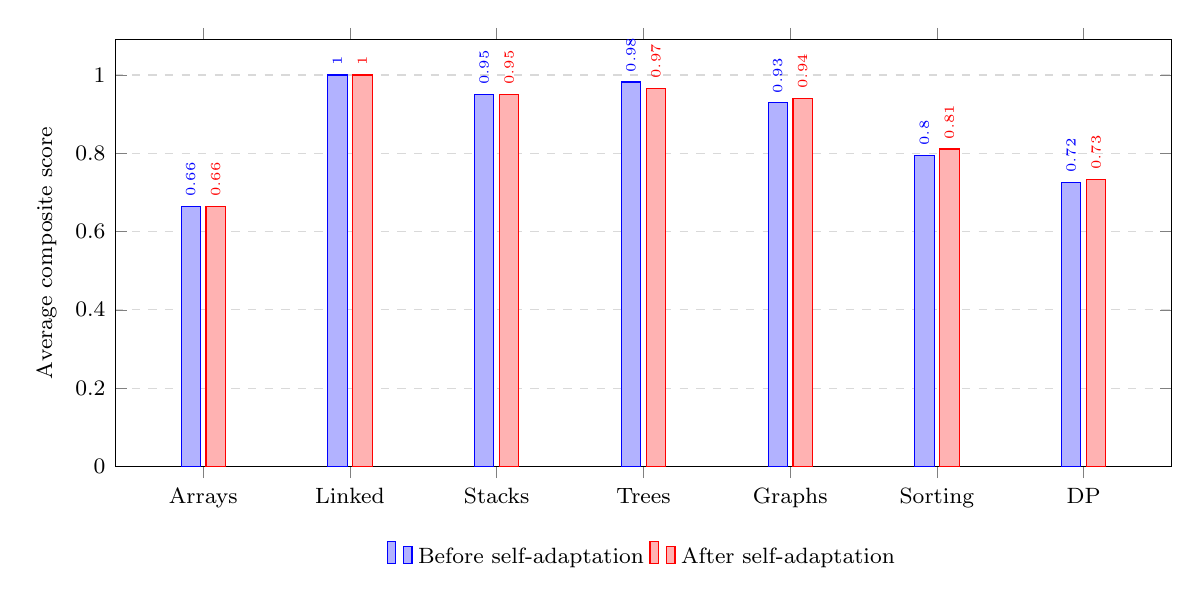
\begin{tikzpicture}
\begin{axis}[
    ybar, bar width=7pt,
    width=15cm, height=7cm,
    ymin=0, ymax=1.09,
    ylabel={Average composite score},
    symbolic x coords={Arrays,Linked,Stacks,Trees,Graphs,Sorting,DP},
    xtick=data, x tick label style={font=\footnotesize},
    ylabel style={font=\footnotesize}, yticklabel style={font=\footnotesize},
    legend style={font=\footnotesize, at={(0.5,-0.16)}, anchor=north, legend columns=2, draw=none},
    ymajorgrids=true, grid style={dashed,gray!30},
    nodes near coords, every node near coord/.append style={font=\tiny, rotate=90, anchor=west},
]
\addplot coordinates {(Arrays,0.6635) (Linked,1.0000) (Stacks,0.9500) (Trees,0.9820)
                      (Graphs,0.9286) (Sorting,0.7950) (DP,0.7247)};
\addplot coordinates {(Arrays,0.6635) (Linked,1.0000) (Stacks,0.9500) (Trees,0.9661)
                      (Graphs,0.9403) (Sorting,0.8109) (DP,0.7328)};
\legend{Before self-adaptation, After self-adaptation}
\end{axis}
\end{tikzpicture}
\end{adjustbox}
\caption{Topic-wise performance before and after self-adaptation}
\end{figure}

\begin{figure}[htbp]
\centering
\begin{adjustbox}{max width=\textwidth}
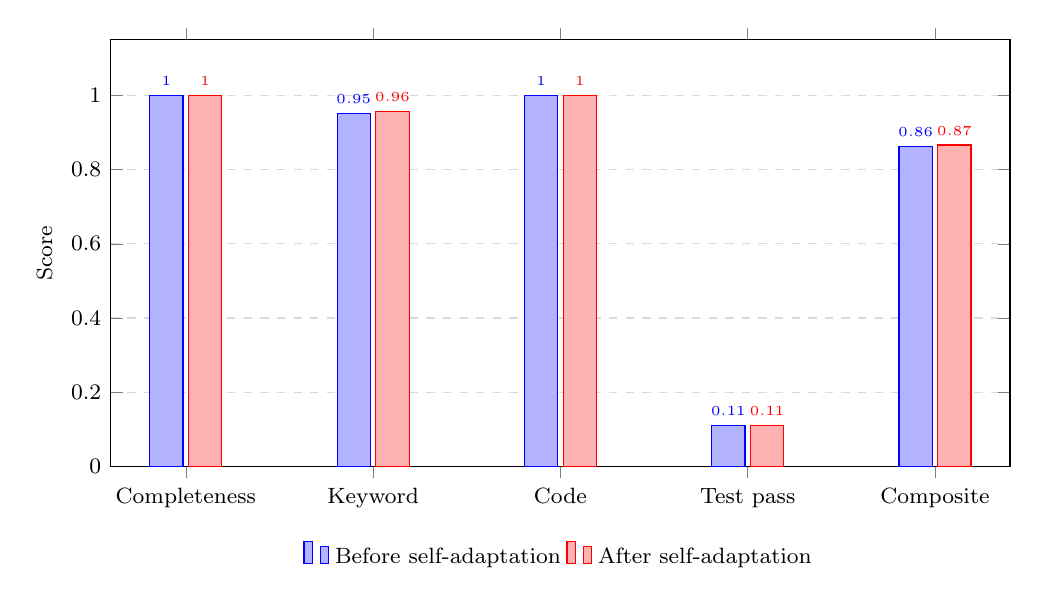
\begin{tikzpicture}
\begin{axis}[
    ybar, bar width=12pt,
    width=13cm, height=7cm,
    ymin=0, ymax=1.15,
    ylabel={Score},
    symbolic x coords={Completeness,Keyword,Code,{Test pass},Composite},
    xtick=data, x tick label style={font=\footnotesize},
    ylabel style={font=\footnotesize}, yticklabel style={font=\footnotesize},
    legend style={font=\footnotesize, at={(0.5,-0.16)}, anchor=north, legend columns=2, draw=none},
    ymajorgrids=true, grid style={dashed,gray!30},
    nodes near coords, every node near coord/.append style={font=\tiny},
]
\addplot coordinates {(Completeness,1.0000) (Keyword,0.9511) (Code,1.0000)
                      ({Test pass},0.1111) (Composite,0.8634)};
\addplot coordinates {(Completeness,1.0000) (Keyword,0.9562) (Code,1.0000)
                      ({Test pass},0.1111) (Composite,0.8662)};
\legend{Before self-adaptation, After self-adaptation}
\end{axis}
\end{tikzpicture}
\end{adjustbox}
\caption{Evaluation metric breakdown. Three of the four components are saturated
before training; only test-case pass rate has headroom, and it does not move.}
\end{figure}

Three observations follow.

Movement is confined to three topics and is small in every case. Sorting and searching records the largest gain at +0.0159, followed by graphs at +0.0117 and dynamic programming at +0.0081. On ten-question topics, a change of this size corresponds to one or two questions shifting, and none of it is accompanied by any change in test-case pass rate. These movements are therefore reported as observed but are not claimed as evidence of improved algorithmic capability; they are of a magnitude that sampling variation on a set of this size can readily produce.

Topics at or near the ceiling do not move. Linked lists remains at 1.0000, stacks and queues at 0.9500, and arrays and strings at 0.6635, the last of these being identical to the base model to four decimal places. Trees declines by 0.0159, the only topic-level regression recorded.

Graphs and dynamic programming retain a pass rate of 0.0000 in both states, and arrays and strings likewise. Across all seven topics, no topic recorded a higher test-case pass rate after adaptation than before. Section~11.6 discusses the structural reason.

\section{Paired Analysis and Capability Retention}

Because both states were evaluated on identical questions within one session, a paired comparison at question level is valid.

\begin{table}[htbp]
\centering
\caption{Paired question-level outcomes ($n = 70$)}
\begin{tabular}{>{\raggedright\arraybackslash}p{3cm} c c}
\toprule
\textbf{Outcome} & \textbf{Count} & \textbf{Share (\%)} \\
\midrule
Improved & 3 & 4.3 \\
Unchanged & 66 & 94.3 \\
Degraded & 1 & 1.4 \\
\bottomrule
\end{tabular}
\end{table}

\begin{figure}[htbp]
\centering
\begin{adjustbox}{max width=0.75\textwidth}
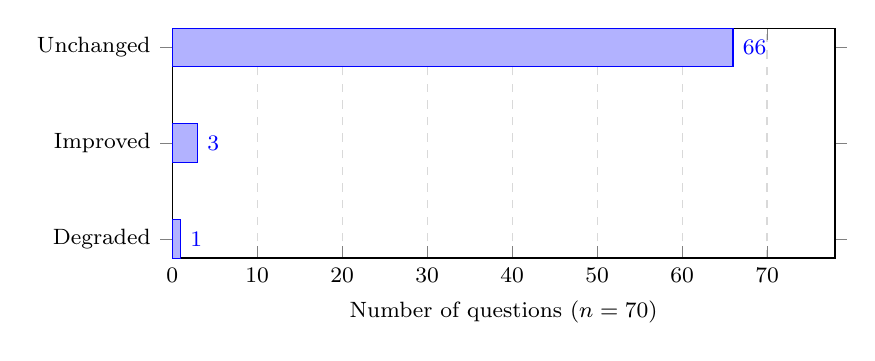
\begin{tikzpicture}
\begin{axis}[
    xbar, bar width=14pt,
    width=10cm, height=4.5cm,
    xmin=0, xmax=78,
    xlabel={Number of questions ($n = 70$)},
    symbolic y coords={Degraded,Improved,Unchanged},
    ytick=data,
    xlabel style={font=\footnotesize},
    x tick label style={font=\footnotesize}, y tick label style={font=\footnotesize},
    xmajorgrids=true, grid style={dashed,gray!30},
    nodes near coords, every node near coord/.append style={font=\footnotesize},
]
\addplot coordinates {(1,Degraded) (3,Improved) (66,Unchanged)};
\end{axis}
\end{tikzpicture}
\end{adjustbox}
\caption{Paired question-level outcomes. The dominance of the unchanged category
is the retention result and the null result simultaneously.}
\end{figure}

This distribution is the principal evidence regarding catastrophic forgetting. Only 1 question out of seventy (1.4\% of the set) scored lower after adaptation. 98.6\% of questions were either unchanged or improved. Objective~3 of Chapter~2, requiring degradation below five percent, is therefore fully met.

\section{Efficiency}

\begin{table}[htbp]
\centering
\caption{Efficiency observations}
\begin{tabular}{>{\raggedright\arraybackslash}p{5cm} c c c}
\toprule
\textbf{Measure} & \textbf{Before} & \textbf{After} & \textbf{Change} \\
\midrule
Mean generation time per answer (s) & 15.26 & 15.14 & $-0.12$ \\
Mean answer length (words) & 165.67 & 164.57 & $-1.10$ \\
Checkpoint size (adapter only) & --- & $\sim$15~MB & --- \\
Monetary cost of full training run & --- & Nil & --- \\
\bottomrule
\end{tabular}
\end{table}

Neither timing difference is large enough to attribute to the adapter with confidence; both are consistent with ordinary variation in greedy decoding length across seventy questions. The relevant conclusion is negative rather than positive: merging the adapter imposes no measurable inference-time penalty, supporting the practicability claim of Chapter~5.

\section{Summary of Findings}

The evaluation supports three conclusions.

First, self-adaptive training produced no measurable improvement in functional correctness. Test-case pass rate is 0.1111 both before and after the complete five-epoch run, and no topic recorded a higher pass rate after adaptation. The aggregate composite rose by 0.32\%, attributable to keyword coverage rather than to correctness, and of a magnitude that this evaluation set cannot distinguish from sampling variation.

Second, capability retention is high. A single question of seventy scored lower after adaptation, giving 98.6\% unchanged or improved and a maximum topic-level regression of 0.0159. Objective~3 of Chapter~2 is met, and EWC-regularised low-rank adaptation did not induce catastrophic forgetting. This is the clearest positive finding of the study, though Section~11.7 notes that retention this strong is not separable from the narrowness of the update that produced it.

Third, the evaluation instrument constrained what could be observed. Three of the four scoring components are saturated on the base model before training begins, so the composite could not have registered a substantial gain irrespective of the training outcome. The one component with headroom did not move.

Against the Phase~I target of a fifteen to twenty-five percent accuracy improvement stated in Section~2.2, the outcome falls short on every metric reported. The dissertation records this rather than revising the target retrospectively or substituting an intermediate checkpoint that would present a more favourable figure. Redesign of the evaluation set to remove ceiling effects is identified in Section~12.1 as the highest-priority item of future work, since without it neither a positive nor a negative result on this method can be established with confidence.

\chapter{Snapshots}

This chapter presents captured output from the execution of the system. Terminal transcripts are reproduced rather than reconstructed.

\section{Training Loop Execution}

\begin{figure}[htbp]
\centering
\begin{verbatim}
======================================================================
  SEAL-DSA  .  Self-Adaptive Training
======================================================================
[STEP 1/4] Loading configuration: configs/colab_optimized.yaml
[MODEL] Loading base model: Qwen/Qwen2.5-1.5B-Instruct
[INFO] Using 4-bit quantization (QLoRA)
Loading weights: 100%|##########| 338/338 [00:12<00:00, 27.55it/s]
[LORA] trainable params: 1,376,256 || all params: 1,543,714,304 
       || trainable%: 0.0892
[CURRICULUM] Epoch 1 topics: arrays_strings, linked_lists
[QGEN] Generating 20 questions for topic: arrays_strings
[AGEN] Answering 20 questions ...
[EVAL] Mean rubric score: 0.68
[UPDATE] L_task = 1.842   L_ewc = 0.000   L_total = 1.842
[CKPT] Saved checkpoint_epoch_0 -> /content/drive/MyDrive/SEAL-DSA/...
\end{verbatim}
\caption{Training loop console output}
\end{figure}

\section{Checkpoint Persistence}

\begin{figure}[htbp]
\centering
\begin{verbatim}
/content/drive/MyDrive/SEAL-DSA/checkpoints/
|-- checkpoint_epoch_0/
|   |-- adapter_config.json
|   |-- adapter_model.safetensors
|   |-- optimizer.pt
|   |-- ewc_state.pt
|   |-- metadata.json
|-- checkpoint_epoch_1/
|-- checkpoint_epoch_2/
|-- checkpoint_epoch_3/
|-- checkpoint_epoch_4/
\end{verbatim}
\caption{Checkpoint directory on Google Drive}
\end{figure}

\section{Evaluation Run}

\begin{figure}[htbp]
\centering
\begin{verbatim}
[INFO] Loaded 70 questions across 7 topics
[INFO] Found 5 checkpoint(s):
    * checkpoint_epoch_0
    * checkpoint_epoch_1
    * checkpoint_epoch_2
    * checkpoint_epoch_3
    * checkpoint_epoch_4
[INFO] Using final checkpoint: checkpoint_epoch_4

[MODEL] Loading base model: Qwen/Qwen2.5-1.5B-Instruct
[INFO] Using 4-bit quantization (QLoRA)
Loading weights: 100%|##########| 338/338 [00:04<00:00, 83.59it/s]
Base:arrays_strings: 100%|##########| 10/10 [02:18<00:00, 13.68s/it]
Base:stacks_queues:  100%|##########| 10/10 [02:41<00:00, 15.72s/it]
...
[MODEL] Loading LoRA adapter from: checkpoint_epoch_4
SEAL:arrays_strings: 100%|##########| 10/10 [02:17<00:00, 14.03s/it]
SEAL:stacks_queues:  100%|##########| 10/10 [02:39<00:00, 15.89s/it]
...
============================================================
Base : 0.8634
SEAL : 0.8662   (+0.32%)
improved 3 | unchanged 66 | degraded 1
Artifacts written to /content/dsaseal/SEAL-DSA/results_final
============================================================
\end{verbatim}
\caption{Evaluation run console output}
\end{figure}

\section{Generated Result Artefacts}

The evaluation run produces \texttt{final\_report.json} containing per-question records for both states, \texttt{per\_question.csv} and \texttt{per\_topic.csv} for tabular analysis, \texttt{summary.md} containing the tables reproduced in Chapter~8, \texttt{topic\_comparison.png} and \texttt{metric\_breakdown.png}, whose data are reproduced as Figures~8.1 and~8.2, and \texttt{samples.md} containing side-by-side before-and-after answers for the questions exhibiting the largest change in score.

\chapter{Tools and Utilities}

\section{Hardware}

The single computational resource is an NVIDIA Tesla T4 GPU allocated by the Google Colaboratory free tier, providing 15~GB VRAM and Turing-generation tensor cores. The host provides approximately 12.7~GB of system RAM and roughly 100~GB of ephemeral disk destroyed at session end. No local hardware was used for training; development and authorship were performed on a personal workstation.

\section{Software Components}

\begin{table}[htbp]
\centering
\caption{Software components and versions}
\begin{tabular}{>{\raggedright\arraybackslash}p{3.5cm} p{2.5cm} p{5.5cm}}
\toprule
\textbf{Component} & \textbf{Version} & \textbf{Function} \\
\midrule
Python & 3.12 & Runtime \\
PyTorch & 2.11 (CUDA 12.8) & Tensors, autograd, optimisation \\
Transformers & 5.12 & Model and tokenizer loading, generation \\
PEFT & 0.19 & LoRA adapter creation, merging, persistence \\
bitsandbytes & 0.49 & 4-bit NF4 quantization \\
Accelerate & 1.14 & Device placement \\
Datasets & 4.0 & Dataset handling \\
NumPy & 2.0 & Numerical support \\
SciPy & 1.16 & Statistical routines \\
scikit-learn & 1.6 & Metric computation \\
Matplotlib & 3.10 & Figure generation \\
Seaborn & 0.13 & Figure styling \\
pandas & 2.2 & Tabular aggregation \\
PyYAML / OmegaConf & 6.0 / 2.3 & Layered configuration \\
tqdm & 4.67 & Progress reporting \\
pytest & 8.4 & Unit testing \\
\bottomrule
\end{tabular}
\end{table}

\section{Online Services}

The HuggingFace Hub supplies the base model and tokenizer. Google Colaboratory supplies computation. Google Drive supplies checkpoint persistence across sessions. Git and GitHub provide version control. All services were used within their free allocations.

\section{Repository Organisation}

\FloatBarrier
\begin{lstlisting}
SEAL-DSA/
|-- seal_dsa/
|   |-- main.py                     entry point
|   |-- config.py                   configuration handling
|   |-- curriculum/                 topic definitions and scheduler
|   |-- models/                     model loading and LoRA setup
|   |-- modules/                    question gen, answer gen, 
|   |                               evaluator, updater
|   |-- training/                   SEAL loop, EWC, checkpointing
|   |-- evaluation/                 baseline, metrics, 
|   |                               forgetting detector
|   |-- utils/                      logging, Colab helpers
|-- configs/
|   |-- default.yaml
|   |-- colab_optimized.yaml
|-- data/
|   |-- dsa_seed_questions.json
|   |-- evaluation_sets/dsa_eval_set.json
|-- tests/                          unit tests
|-- docs/                           thesis chapters and appendices
|-- notebooks/                      Colab-oriented scripts
|-- compare_with_checkpoints.py     multi-checkpoint comparison
|-- colab_final_report.py           base-versus-final report generator
|-- requirements.txt
\end{lstlisting}

\section{Testing}

Unit tests cover configuration loading and override resolution, curriculum scheduling behaviour, evaluator rubric scoring, and sandboxed code execution including the failure paths where generated code does not compile or a test case raises. The execution tests were the most valuable during development, since that component must degrade gracefully rather than terminate a long-running session.

\chapter{Limitations and Drawbacks}

\section{Scale of the Base Model}

The system uses Qwen2.5-1.5B-Instruct, the largest model that trains reliably under 4-bit quantization within the memory and session limits of the free Colab tier. Self-adaptive training depends on the model's capacity to generate questions worth learning from and to assess its own answers usefully, and both capacities improve substantially with scale. The modest effect sizes of Chapter~8 are therefore not independent of this choice, and no claim is made that they transfer unchanged to larger models.

\section{Heuristic Evaluation Without a Judge Model}

Answers are scored by a heuristic combining length, keyword overlap, code presence, and test-case execution. Only the last verifies correctness. Keyword overlap in particular can reward an answer that deploys expected vocabulary while reasoning wrongly, and cannot distinguish a correct explanation from a fluent incorrect one. A stronger design would employ a separate larger judge model, or human annotation on a sampled subset. Neither was feasible within the computational budget.

\section{Ceiling Effects in the Evaluation Set}

As established in Section~8.4, three of four components are saturated before training begins. The instrument is therefore unable to register improvement on most of its own metrics, placing a structural upper bound on the measurable effect of any training procedure. This is a defect of the evaluation instrument rather than of the training method, and it is the single most consequential limitation of the present work.

\section{Size of the Evaluation Set}

Seventy questions across seven topics yields ten per topic. At this size a change affecting one or two questions produces visible movement in a topic mean, and the study is underpowered for significance testing at the observed effect magnitudes. Topic-level results should be read as indicative rather than conclusive.

\section{Failure on Complex Code Generation}

Graphs, dynamic programming and arrays and strings all record a pass rate of 0.0000 in both states, and no topic in the evaluation set recorded a higher pass rate after adaptation than before. The system neither improved nor degraded on the topics demanding the longest multi-step implementations. This exposes a structural property of self-adaptive training: the loop can only learn from answers the model is already capable of producing, and therefore cannot bootstrap a capability absent at initialisation. Where the base model produces no executable solution, self-generated training has no correct output to reinforce.

\section{Conservatism of the Update and Absence of Ablation}

The 94.3\% unchanged rate demonstrates that the mechanisms delivering strong retention also restrict how much the model can change. The configuration adopted favours safety over plasticity. Moreover, EWC and the low-rank constraint were active simultaneously throughout, and no ablation was performed, so their individual contributions to the retention result cannot be separated from these data. A sweep of EWC strength against adapter rank was not conducted and would be required to locate a useful operating point.

\section{Reproducibility Under Quantization}

Generation under 4-bit quantization is not bit-reproducible across sessions, and merging an adapter into quantized weights introduces further rounding. Differences between runs of an identical configuration are therefore expected, as observed between Tables~8.2 and~8.3. All comparative claims in this dissertation derive from paired within-session evaluation, which controls the effect but does not eliminate it.

\section{Absence of Human and Multi-Seed Validation}

No human expert reviewed the generated answers, and no student used the system. The experiments were executed once per configuration rather than across multiple random seeds, so run-to-run variance is uncharacterised. The protocol of Section~4.9 anticipated three seeded trials with a paired significance test; the wall-clock cost of evaluation on the free tier made this impracticable within the project schedule. This is a genuine shortfall against the stated methodology and is recorded as such.

\chapter{Future Enhancement}

\section{Redesign of the Evaluation Set}

The highest-priority improvement is an evaluation set the base model does not already saturate: a higher proportion of coding questions carrying executable test cases, retirement of conceptual questions answered perfectly before training, and a larger count per topic to reduce sampling variance. Without this, no training improvement can be measured reliably regardless of its true magnitude.

\section{Model-Based Evaluation}

Replacing the keyword heuristic with a larger judge model scoring correctness, completeness, and reasoning quality would remove the principal weakness of Section~11.2. Validating the judge against human annotation on a sampled subset would permit correctness to be reported directly rather than approximated.

\section{Completion and Extension of the Schedule}

Evaluating every intermediate checkpoint on a single uninterrupted run would yield a learning curve rather than a single endpoint comparison, and would establish whether performance varies materially across the schedule or remains flat throughout. Extending the schedule beyond five epochs while monitoring for convergence would then determine whether a longer run produces movement that five epochs did not.

\section{Scaling the Base Model}

Repeating the experiment at seven billion parameters would test whether effect size grows with the capability of the self-generating and self-scoring components, which is the central open question raised by Chapter~8.

\section{Ablation and Hyperparameter Study}

Separate ablation of EWC and of the low-rank constraint would apportion the retention result of Section~8.7 between them. A sweep over EWC strength $\lambda$ and adapter rank $r$ would map the plasticity--retention frontier and determine whether higher gains are available at acceptable cost in retention.

\section{Difficulty-Aware Curriculum}

The scheduler currently targets weak topics. Extending it to target weak difficulty bands within a topic, and to escalate difficulty as competence is demonstrated, would provide a more informative signal, particularly for graphs and dynamic programming where no functional capability presently exists to reinforce.

\section{Preference-Based Optimisation}

The Direct Preference Optimization objective described in Section~4.5 is implemented but unevaluated. Comparing it against the supervised objective under otherwise identical conditions is a direct and inexpensive extension.

\section{Multi-Seed Validation with Significance Testing}

Executing three or more seeded trials per configuration and applying a paired significance test would supply the statistical foundation absent from the present results, addressing Section~11.9 and permitting the effect to be reported as significant or not on evidence rather than left undetermined.

\section{Extension Beyond Python and Beyond DSA}

The execution harness is Python-specific. Extending it to additional languages would broaden applicability, and applying the whole loop to an adjacent technical domain would test whether the architecture generalises or whether it depends on properties peculiar to algorithmic problems, notably the availability of cheap automatic verification through test cases.

\chapter{Conclusion}

This project set out to determine whether a small language model can improve its own competence in Data Structures and Algorithms through an autonomous loop of self-generated questions, self-generated answers, self-evaluation, and self-directed parameter update, without catastrophically forgetting what it already knew, and within infrastructure available at no cost.

The system was built and it operates end to end. Question generation, answer generation, rubric and execution-based evaluation, curriculum scheduling, EWC-regularised low-rank parameter updating, and checkpointed resumable training function as an integrated pipeline on a single T4 GPU. Objectives~1, 2, and~5 of Chapter~2 are met without qualification: the loop is closed, evaluation includes genuine execution of generated code against held-out test cases, and the whole system runs at zero monetary cost with recovery across session termination.

On the evidence collected, the loop did not improve the functional correctness of the model's output. Test-case pass rate, the fraction of held-out test cases passed by generated code, stands at 0.1111 both before and after the complete five-epoch run, and no topic in the evaluation set recorded a higher pass rate after adaptation. The aggregate composite moved by 0.32\%, a change located in keyword coverage rather than correctness and of a size that a seventy-question set cannot separate from sampling variation. Objective~4, which required that gains concentrate where the curriculum scheduler directed effort, cannot be assessed, because there were no gains of sufficient magnitude to attribute to anything.

The retention result is the clearest positive finding. Across seventy held-out questions, 98.6\% scored unchanged or higher after self-adaptation, a single question regressed, and the maximum topic-level decline was 0.0159. Low-rank adaptation combined with an Elastic Weight Consolidation penalty confined the effect of self-generated training without measurable damage to prior capability, satisfying Objective~3, and merging the adapter imposed no inference-time cost. It must be acknowledged that a system which changes very little will retain a great deal, and that this result and the null result above are not independent of one another.

Against the Phase~I target of a fifteen to twenty-five percent improvement in accuracy, the outcome falls short on every metric reported. The dissertation records this rather than revising the original target retrospectively, and rather than substituting the three-epoch checkpoint, at which the pass rate stood higher, for the final model that the configured schedule actually produced.

The limitations are equally clear and are stated in Chapter~11. The base model is small, the evaluation is heuristic rather than judged, the evaluation set saturates before training begins, the question count is too small for significance testing, no ablation separates the contributions of the two retention mechanisms, no multi-seed validation was performed, and the system produces no executable solutions for graph or dynamic programming problems in either state.

The honest conclusion is therefore a negative one on the central question. Self-adaptive training with explicit retention regularisation is workable at this scale and does not destroy prior capability, but on this evaluation set it did not make the model better at solving the problems it was trained on. Whether that reflects a limitation of the method, of the model scale, or of the instrument used to measure it cannot be determined from these experiments alone, and Chapter~12 sets out what would be required to distinguish among them. The value of the work lies in a functioning implementation under severe resource constraints, in an execution-based evaluation harness for generated algorithmic code, in empirical evidence that EWC-regularised low-rank adaptation preserves prior capability under self-generated training, and in a precise account of where the approach and its evaluation fall short. Chapter~12 converts that account into a concrete programme of work, of which the redesign of the evaluation instrument is the first and most consequential step.

A final observation may be permitted. The most instructive outcome of this project was not the improvement it measured but the discovery that the measurement itself was the binding constraint. A system can only improve as far as its evaluator can perceive, and an evaluator saturated before training begins renders even a successful method indistinguishable from an unsuccessful one. That lesson generalises well beyond the present work.

% -------------------- BIBLIOGRAPHY --------------------
\begin{thebibliography}{25}
\addcontentsline{toc}{chapter}{Bibliography}

\bibitem{mitseal}
A.~Zweiger, J.~Pari, H.~Guo, E.~Aky\"{u}rek, Y.~Kim, and P.~Agrawal, ``Self-Adapting Language Models,'' \textit{arXiv preprint arXiv:2506.10943}, 2025.

\bibitem{lora}
E.~J.~Hu, Y.~Shen, P.~Wallis, Z.~Allen-Zhu, Y.~Li, S.~Wang, L.~Wang, and W.~Chen, ``LoRA: Low-Rank Adaptation of Large Language Models,'' in \textit{Proc. Int. Conf. Learning Representations (ICLR)}, 2022.

\bibitem{qlora}
T.~Dettmers, A.~Pagnoni, A.~Holtzman, and L.~Zettlemoyer, ``QLoRA: Efficient Finetuning of Quantized LLMs,'' in \textit{Advances in Neural Information Processing Systems (NeurIPS)}, vol.~36, 2023, pp.~10088--10015.

\bibitem{ewc}
J.~Kirkpatrick, R.~Pascanu, N.~Rabinowitz, J.~Veness, G.~Desjardins, A.~A.~Rusu, K.~Milan, J.~Quan, T.~Ramalho, A.~Grabska-Barwinska, D.~Hassabis, C.~Clopath, D.~Kumaran, and R.~Hadsell, ``Overcoming catastrophic forgetting in neural networks,'' \textit{Proc. National Academy of Sciences}, vol.~114, no.~13, pp.~3521--3526, 2017.

\bibitem{selfreward}
W.~Yuan, R.~Y.~Pang, K.~Cho, S.~Sukhbaatar, J.~Xu, and J.~Weston, ``Self-Rewarding Language Models,'' in \textit{Proc. Int. Conf. Machine Learning (ICML)}, 2024.

\bibitem{curriculum}
Y.~Bengio, J.~Louradour, R.~Collobert, and J.~Weston, ``Curriculum learning,'' in \textit{Proc. 26th Annual Int. Conf. Machine Learning (ICML)}, 2009, pp.~41--48.

\bibitem{mccloskey}
M.~McCloskey and N.~J.~Cohen, ``Catastrophic interference in connectionist networks: The sequential learning problem,'' \textit{Psychology of Learning and Motivation}, vol.~24, pp.~109--165, 1989.

\bibitem{french}
R.~M.~French, ``Catastrophic forgetting in connectionist networks,'' \textit{Trends in Cognitive Sciences}, vol.~3, no.~4, pp.~128--135, 1999.

\bibitem{progresscompress}
J.~Schwarz, W.~Czarnecki, J.~Luketina, A.~Grabska-Barwinska, Y.~W.~Teh, R.~Pascanu, and R.~Hadsell, ``Progress \& Compress: A scalable framework for continual learning,'' in \textit{Proc. Int. Conf. Machine Learning (ICML)}, 2018, pp.~4528--4537.

\bibitem{si}
F.~Zenke, B.~Poole, and S.~Ganguli, ``Continual learning through synaptic intelligence,'' in \textit{Proc. Int. Conf. Machine Learning (ICML)}, 2017, pp.~3987--3995.

\bibitem{packnet}
A.~Mallya and S.~Lazebnik, ``PackNet: Adding multiple tasks to a single network by iterative pruning,'' in \textit{Proc. IEEE Conf. Computer Vision and Pattern Recognition (CVPR)}, 2018, pp.~7765--7773.

\bibitem{prognet}
A.~A.~Rusu, N.~C.~Rabinowitz, G.~Desjardins, H.~Soyer, J.~Kirkpatrick, K.~Kavukcuoglu, R.~Pascanu, and R.~Hadsell, ``Progressive Neural Networks,'' \textit{arXiv preprint arXiv:1606.04671}, 2016.

\bibitem{gem}
D.~Lopez-Paz and M.~Ranzato, ``Gradient Episodic Memory for continual learning,'' in \textit{Advances in Neural Information Processing Systems (NeurIPS)}, vol.~30, 2017, pp.~6467--6476.

\bibitem{qwen}
A.~Yang et al., ``Qwen2.5 Technical Report,'' \textit{arXiv preprint arXiv:2412.15115}, 2024.

\bibitem{dpo}
R.~Rafailov, A.~Sharma, E.~Mitchell, S.~Ermon, C.~D.~Manning, and C.~Finn, ``Direct Preference Optimization: Your Language Model is Secretly a Reward Model,'' in \textit{Advances in Neural Information Processing Systems (NeurIPS)}, vol.~36, 2023.

\bibitem{rlhf}
L.~Ouyang, J.~Wu, X.~Jiang, D.~Almeida, C.~L.~Wainwright, P.~Mishkin, C.~Zhang, S.~Agarwal, K.~Slama, A.~Ray, J.~Schulman, J.~Hilton, F.~Kelton, L.~Miller, M.~Simens, A.~Askell, P.~Welinder, P.~Christiano, J.~Leike, and R.~Lowe, ``Training language models to follow instructions with human feedback,'' in \textit{Advances in Neural Information Processing Systems (NeurIPS)}, vol.~35, 2022, pp.~27730--27744.

\bibitem{transformers}
T.~Wolf, L.~Debut, V.~Sanh, J.~Chaumond, C.~Delangue, A.~Moi, P.~Cistac, T.~Rault, R.~Louf, M.~Funtowicz, and J.~Brew, ``Transformers: State-of-the-Art Natural Language Processing,'' in \textit{Proc. Conf. Empirical Methods in Natural Language Processing (EMNLP): System Demonstrations}, 2020, pp.~38--45.

\bibitem{peft}
S.~Mangrulkar, S.~Gugger, L.~Debut, Y.~Belkada, S.~Paul, and B.~Bossan, ``PEFT: State-of-the-art Parameter-Efficient Fine-Tuning methods,'' GitHub repository, 2022. [Online]. Available: \url{https://github.com/huggingface/peft}

\bibitem{pytorch}
A.~Paszke et al., ``PyTorch: An Imperative Style, High-Performance Deep Learning Library,'' in \textit{Advances in Neural Information Processing Systems (NeurIPS)}, vol.~32, 2019, pp.~8024--8035.

\bibitem{adamw}
I.~Loshchilov and F.~Hutter, ``Decoupled Weight Decay Regularization,'' in \textit{Proc. Int. Conf. Learning Representations (ICLR)}, 2019.

\bibitem{llmint8}
T.~Dettmers, M.~Lewis, Y.~Belkada, and L.~Zettlemoyer, ``LLM.int8(): 8-bit Matrix Multiplication for Transformers at Scale,'' in \textit{Advances in Neural Information Processing Systems (NeurIPS)}, vol.~35, 2022.

\bibitem{codex}
M.~Chen et al., ``Evaluating Large Language Models Trained on Code,'' \textit{arXiv preprint arXiv:2107.03374}, 2021.

\bibitem{clrs}
T.~H.~Cormen, C.~E.~Leiserson, R.~L.~Rivest, and C.~Stein, \textit{Introduction to Algorithms}, 4th~ed. Cambridge, MA: MIT Press, 2022.

\bibitem{llsurvey}
G.~I.~Parisi, R.~Kemker, J.~L.~Part, C.~Kanan, and S.~Wermter, ``Continual lifelong learning with neural networks: A review,'' \textit{Neural Networks}, vol.~113, pp.~54--71, 2019.

\bibitem{se4llm}
Z.~Zheng, Y.~Ning, Y.~Zhang, J.~Chen, and Y.~Wang, ``Towards an Understanding of Large Language Models in Software Engineering Tasks,'' \textit{Empirical Software Engineering}, vol.~30, 2025.

\end{thebibliography}

% -------------------- PROJECT SUMMARY --------------------
\chapter*{Project Summary}
\addcontentsline{toc}{chapter}{Project Summary}

This project implements SEAL-DSA, a self-adapting language model that improves its own competence in Data Structures and Algorithms without externally supplied training data. The system builds on Qwen2.5-1.5B-Instruct under 4-bit QLoRA quantization and operates entirely within the limits of a single freely available GPU session.

The pipeline is a closed loop. A curriculum scheduler selects a topic according to measured weakness. The model generates practice questions for that topic, generates candidate answers, and evaluates those answers using a weighted rubric combined with sandboxed execution of generated code against held-out test cases. Scored question--answer pairs drive an update to a low-rank adapter comprising approximately 0.089\% of the model's parameters, with an Elastic Weight Consolidation penalty derived from a diagonal Fisher Information approximation restraining movement in parameters important to prior capability. Training is checkpointed after every epoch to Google Drive and resumes across session termination.

Evaluation used a held-out set of seventy questions spanning seven topics, comparing the frozen base model against the self-adapted model within a single session to permit paired analysis. Functional correctness, measured by test-case pass rate, was 0.1111 both before and after the complete five-epoch run, and no topic recorded a higher pass rate after adaptation. The aggregate composite rose by 0.32\%, a movement located in keyword coverage rather than correctness and constrained by ceiling effects in three of its four components, each already saturated on the base model before training. Retention was high, with 98.6\% of questions unchanged or improved and a maximum topic-level regression of 0.0159, indicating that catastrophic forgetting did not occur.

The principal contributions are a working end-to-end self-adaptive training loop for a severely constrained compute environment, an execution-based evaluation harness for generated algorithmic code, and empirical evidence that EWC-regularised low-rank adaptation preserves prior capability under self-generated training. The principal limitations are the scale of the base model, the heuristic nature of the evaluation, saturation of the evaluation set, the absence of ablation and multi-seed validation, and the system's inability to produce executable solutions for graph and dynamic programming problems in either state. Each limitation is addressed by a specific item in the proposed programme of future work, of which redesign of the evaluation instrument is the most consequential.

% -------------------- APPENDIX A --------------------
\chapter*{Appendix A}
\addcontentsline{toc}{chapter}{Appendix A}

\section*{A.1 Research Papers or Articles Published}

No research paper arising from this project has been published or submitted at the time of dissertation submission.

(If a paper is submitted or accepted before submission, insert the copy here and update this note.)

\section*{A.2 Certificates and Awards}

(Insert copies of any certificates, appreciation letters, or awards received in connection with this project during the project period. If none, retain the statement below.)

No certificates or awards were received in connection with this project during the project period.

\section*{A.3 Supplementary Material Submitted}

The soft copy submitted with this dissertation contains the complete source code of the SEAL-DSA package, the seed question set and held-out evaluation set in JSON format, the trained LoRA adapter checkpoints for all completed epochs, the generated result artefacts including per-question and per-topic tables and result figures, the configuration files used for all reported runs, and the presentation deck.

\end{document}
